%  LaTeX support: latex@mdpi.com 
%  For support, please attach all files needed for compiling as well as the log file, and specify your operating system, LaTeX version, and LaTeX editor.

%=================================================================
\documentclass[journal,article,submit,moreauthors]{Definitions/mdpi} 
%\documentclass[preprints,article,submit,moreauthors]{Definitions/mdpi} 
% For posting an early version of this manuscript as a preprint, you may use "preprints" as the journal. Changing "submit" to "accept" before posting will remove line numbers.

%--------------------
% Class Options:
%--------------------
%----------
% journal
%----------
% Choose between the following MDPI journals:
% accountaudit, acn, acoustics, actuators, addictions, addictprev, adhesives, adolescents, aerobiology, aerospace, agriculture, agriengineering, agrochemicals, agronomy, ai, aichem, aieng, aimater, aimed, aipa, air, aisens, aisoc, algorithms, allergies, alloys, amh, analog, analytica, analytics, anatomia, anesthres, animals, antibiotics, antibodies, antioxidants, applbiosci, appliedchem, appliedmath, appliedphys, applmech, applmicrobiol, applnano, applsci, aps, aquacj, archaeolstud, architecture, arm, arthropoda, asc, asi, astronautics, astronomy, atmosphere, atoms, audiolres, automation, axioms, bacteria, batteries, bdcc, beverages, biochem, bioengineering, biologics, biology, biomass, biomechanics, biomed, biomedicines, biomedinformatics, biomimetics, biomolecules, biophysica, bioresourbioprod, biosensors, biosphere, biotech, birds, blockchains, bloods, blsf, brainsci, breath, buildings, cancers, carbon, cardio, cardiogenetics, cardiovascmed, catalysts, cells, ceramics, challenges, chemengineering, chemistry, chemosensors, chemproc, children, chips, cimb, civileng, cleantechnol, climate, clinbioenerg, clinpract, clockssleep, cmd, cmtr, coasts, coatings, colloids, colorants, commodities, complexities, complications, compounds, computation, computers, condensedmatter, conservation, constrmater, cosmetics, covid, crops, cryo, cryptography, crystals, csmf, ctn, culture, curroncol, cyber, dairy, data, ddc, dentistry, dermato, dermatopathology, designs, devices, dhi, diabetology, diagnostics, dietetics, digital, disabilities, diseases, diversity, dna, drones, drugreact, drylands, dynamics, earth, ebj, ecm, ecologies, edm, eesp, electricity, electrochem, electronicmat, electronics, embodiedintell, encyclopedia, endocrines, energies, eng, engproc, entomology, entropy, environments, environremediat, epidemiologia, epigenomes, esa, est, fermentation, fibers, fintech, fire, fishes, fluids, foodeng, foods, forecasting, forensicsci, forests, fossstud, foundations, fractalfract, freshwater, fuels, future, futureinternet, futurepharmacol, futurephys, futuretransp, galaxies, gases, gastroent, gastrointestdisord, gastronomy, gels, genes, geochem, geographies, geohazards, geomatics, geometry, geosciences, geotechnics, geriatrics, germs, glacies, grainsci, grasses, green, greenhealth, gucdd, gynecolcancer, hardware, hazardousmatters, healthcare, healthcmater, hearts, hemato, hematolrep, hep, heritage, higheredu, highthroughput, horticulturae, hospitals, hydrobiology, hydrogen, hydrology, hydrometeorology, hydropower, hygiene, idr, iic, ijem, ijerph, ijgi, ijmd, ijms, ijns, ijom, ijp, ijpb, ijt, ijtm, ijtpp, ijtst, ime, immuno, industries, inflammj, informatics, information, infrastructures, inorganics, insects, instruments, inventions, iot, j, jaestheticmed, jal, japma, jcdd, jcm, jcp, jcrm, jcs, jcto, jdad, jdb, jdream, jemr, jeta, jfb, jfmk, jfth, jgbg, jgg, jimaging, jlpea, jmahp, jmmp, jmms, jmp, jmse, jne, jnt, jof, joi, joitmc, joma, jop, joptm, jor, jox, jpbi, jphytomed, jpm, jsan, jtaer, jvd, jzbg, kidneydial, kinasesphosphatases, knowledge, labmed, laboratories, lam, land, lasers, legumes, life, lights, limnolrev, lipidology, liquids, livers, logics, logistics, lubricants, lymphatics, machines, macromol, magnetism, magnetochemistry, make, marinedrugs, maritime, materials, materproc, mathematics, mca, mcb, measurements, medicina, medicines, medsci, membranes, merits, metabolites, metals, meteorology, methane, metrics, metrology, micro, microarrays, microbiolres, microelectronics, micromachines, microorganisms, microplastics, microwave, minerals, mining, mmphys, modelling, molbank, molecules, mollusca, mps, msf, mti, multimedia, muscles, nanoenergyadv, nanomanufacturing, nanomaterials, ncrna, ndt, network, neuroglia, neuroimaging, neurolint, neurosci, nitrogen, notspecified, nursrep, nutraceuticals, nutrients, obesities, occuphealth, oceans, ohbm, onco, optics, oral, organics, organoids, osteology, oxygen, pandemics, parasites, parasitologia, particles, pathogens, pathophysiology, pediatrrep, pets, pharmaceuticals, pharmaceutics, pharmacoepidemiology, pharmacy, phc, philosophies, photochem, photonics, photovoltaics, phycology, physchem, physics, physiologia, plants, plasma, platforms, pollutants, polymers, polysaccharides, populations, poultry, powders, precision, precisoncol, preprints, proceedings, processes, prosthesis, proteomes, psf, psychiatryint, psychoactives, purification, quantumrep, quaternary, qubs, radiation, rareearths, rdt, reactions, realestate, receptors, recycling, regeneration, remotesensing, reports, reprodmed, resources, rheumato, rjpm, robotics, rsee, ruminants, safety, sanpp, sca, sci, scipharm, sclerosis, seeds, sensors, separations, sexes, shi, signals, sinusitis, siuj, skins, smartcities, smartfish, sna, societies, software, soilsystems, solar, solids, spectroscj, sports, standards, stats, std, stratsediment, stresses, strokerep, superintelligence, surfaces, surgeries, suschem, sustainability, sustainfoods, sustainpackag, symmetry, synbio, systems, tae, targets, taxonomy, technologies, telecom, test, textiles, thalassrep, therapeutics, thermo, timespace, tomography, toxics, toxins, tph, transplantology, transportation, traumacare, traumas, tri, tropicalmed, universe, urbansci, uro, vaccines, vehicles, venereology, vetsci, vibration, virtualworlds, viruses, vision, waste, water, welding, wem, wevj, wild, wind, women, world, zoonoticdis

%---------
% article
%---------
% The default type of manuscript is "article", but can be replaced by: 
% abstract, addendum, article, benchmark, book, bookreview, briefcommunication, briefreport, casereport, changes, clinicopathologicalchallenge, comment, commentary, communication, conceptpaper, conferenceproceedings, correction, conferencereport, creative, datadescriptor, discussion, entry, expressionofconcern, extendedabstract, editorial, essay, erratum, fieldguide, hypothesis, interestingimages, letter, meetingreport, monograph, newbookreceived, obituary, opinion, proceedingpaper, projectreport, reply, retraction, review, perspective, protocol, shortnote, studyprotocol, supfile, systematicreview, technicalnote, viewpoint, guidelines, registeredreport, tutorial,  giantsinurology, urologyaroundtheworld
% supfile = supplementary materials

%----------
% submit
%----------
% The class option "submit" will be changed to "accept" by the Editorial Office when the paper is accepted. This will only make changes to the frontpage (e.g., the logo of the journal will get visible), the headings, and the copyright information. Also, line numbering will be removed. Journal info and pagination for accepted papers will also be assigned by the Editorial Office.

%------------------
% moreauthors
%------------------
% If there is only one author the class option oneauthor should be used. Otherwise use the class option moreauthors.

%=================================================================
% MDPI internal commands - do not modify
\firstpage{1} 
\makeatletter 
\setcounter{page}{\@firstpage} 
\makeatother
\pubvolume{1}
\issuenum{1}
\articlenumber{0}
\pubyear{2026}
\copyrightyear{2026}
%\externaleditor{Firstname Lastname} % More than 1 editor, please add `` and '' before the last editor name
\datereceived{ } 
\daterevised{ } % Comment out if no revised date
\dateaccepted{ } 
\datepublished{ } 
%\datecorrected{} % For corrected papers: "Corrected: XXX" date in the original paper.
%\dateretracted{} % For retracted papers: "Retracted: XXX" date in the original paper.
%\doinum{} % Used for some special journals, like molbank
%\pdfoutput=1 % Uncommented for upload to arXiv.org
%\CorrStatement{yes}  % For updates
%\longauthorlist{yes} % For many authors that exceed the left citation part
%\IsAssociation{yes} % For association journals

%=================================================================
% Add packages and commands here. The following packages are loaded in our class file: fontenc, inputenc, calc, indentfirst, fancyhdr, graphicx, epstopdf, lastpage, ifthen, float, amsmath, amssymb, lineno, setspace, enumitem, mathpazo, booktabs, titlesec, etoolbox, tabto, xcolor, colortbl, soul, multirow, microtype, tikz, totcount, changepage, attrib, upgreek, array, tabularx, pbox, ragged2e, tocloft, marginnote, marginfix, enotez, amsthm, natbib, hyperref, cleveref, scrextend, url, geometry, newfloat, caption, draftwatermark, seqsplit
% cleveref: load \crefname definitions after \begin{document}

\usepackage{algorithm}
\usepackage{algpseudocode}
\usepackage{wrapfig}
\usetikzlibrary{arrows.meta, positioning}

%=================================================================
% Please use the following mathematics environments: Theorem, Lemma, Corollary, Proposition, Characterization, Property, Problem, Example, ExamplesandDefinitions, Hypothesis, Remark, Definition, Notation, Assumption
%% For proofs, please use the proof environment (the amsthm package is loaded by the MDPI class).

%=================================================================
% Full title of the paper (Capitalized)
\Title{A Framework for Global Background Subtraction in Fiber Diffraction Patterns from Striated Muscle}

% Author Orchid ID: enter ID or remove command
\newcommand{\orcidauthorA}{0009-0006-3713-2834} % Add \orcidA{} behind the author's name
\newcommand{\orcidauthorB}{0000-0001-7805-1527} % Add \orcidB{} behind the author's name
\newcommand{\orcidauthorC}{0000-0003-4848-3323} % Add \orcidC{} behind the author's name

% Authors, for the paper (add full first names)
\Author{Irina Klein $^{1}$\orcidA{}, Gady Agam $^{1}$\orcidB{} and Thomas Irving $^{2,}$\orcidC{}*}

%\longauthorlist{yes}

% MDPI internal command: Authors, for metadata in PDF
\AuthorNames{Irina Klein, Gady Agam and Thomas Irving}

% Affiliations / Addresses (Add [1] after \address if there is only one affiliation.)
\address{%
$^{1}$ \quad Computer Science Department, Illinois Institute of Technology, Chicago, IL 60616, USA\\
$^{2}$ \quad Biology Department, Illinois Institute of Technology, Chicago, IL 60616, USA}

% Contact information of the corresponding author
\corres{Correspondence: iklein@illinoistech.edu (I.K.); irving@illinoistech.edu  (T.C.I.)}

% Current address and/or shared authorship
%\firstnote{Current address: Affiliation.}  
% Current address should not be the same as any items in the Affiliation section.

%\secondnote{These authors contributed equally to this work.}
% The commands \thirdnote{} till \eighthnote{} are available for further notes.

%\simplesumm{} % Simple summary

%\conference{} % An extended version of a conference paper

% Abstract (Do not insert blank lines, i.e. \\) 
\abstract{Accurate background subtraction is critical for analyzing X-ray fiber diffraction patterns from striated muscle, where diffuse scattering, instrumental artifacts, and specimen-dependent features complicate the separation of signal from background. Existing methods are often applied heuristically, with limited guidance on parameter selection or objective evaluation, leading to variability in downstream analyses. We present a unified framework for evaluating and optimizing background subtraction methods for muscle fiber diffraction images. It combines physically motivated image-quality metrics, synthetic signal validation, and global optimization to identify method-specific parameters that balance background suppression with signal preservation, enabling direct quantitative comparison of commonly used approaches within a consistent pipeline. Applied to synchrotron diffraction patterns from striated muscle, optimized parameters substantially improve background removal consistency and reduce artifacts relative to default or ad hoc settings, while preserving key features such as equatorial reflections and layer lines. The aggregate loss correlates with expert visual assessment, and individual metrics reveal characteristic failure modes of different subtraction strategies. We additionally evaluate parametric fitting of the equatorial streak combined with background removal. The framework provides an objective, reproducible basis for selecting and tuning background subtraction methods, supporting more reliable quantitative analysis of synchrotron muscle fiber diffraction experiments.}

% Keywords
\keyword{background subtraction, synchrotron X-ray diffraction, fiber diffraction, striated muscle, quantitative evaluation, image analysis} 

% The fields PACS, MSC, and JEL may be left empty or commented out if not applicable
%\PACS{J0101}
%\MSC{}
%\JEL{}

%%%%%%%%%%%%%%%%%%%%%%%%%%%%%%%%%%%%%%%%%%
% Only for the journal Diversity
%\LSID{\url{http://}}

%%%%%%%%%%%%%%%%%%%%%%%%%%%%%%%%%%%%%%%%%%
% Only for the journal Applied Sciences
%\featuredapplication{Authors are encouraged to provide a concise description of the specific application or a potential application of the work. This section is not mandatory.}
%%%%%%%%%%%%%%%%%%%%%%%%%%%%%%%%%%%%%%%%%%

%%%%%%%%%%%%%%%%%%%%%%%%%%%%%%%%%%%%%%%%%%
% Only for the journal Data
%\dataset{DOI number or link to the deposited data set if the data set is published separately. If the data set shall be published as a supplement to this paper, this field will be filled by the journal editors. In this case, please submit the data set as a supplement.}
%\datasetlicense{License under which the data set is made available (CC0, CC-BY, CC-BY-SA, CC-BY-NC, etc.)}

%%%%%%%%%%%%%%%%%%%%%%%%%%%%%%%%%%%%%%%%%%
% Only for the journal BioTech, Fishes, Neuroimaging and Toxins
%\keycontribution{The breakthroughs or highlights of the manuscript. Authors can write one or two sentences to describe the most important part of the paper.}

%%%%%%%%%%%%%%%%%%%%%%%%%%%%%%%%%%%%%%%%%%
% Only for the journal Encyclopedia
%\encyclopediadef{For entry manuscripts only: please provide a brief overview of the entry title instead of an abstract.}

%%%%%%%%%%%%%%%%%%%%%%%%%%%%%%%%%%%%%%%%%%
% Different journals have different requirements. Please check the specific journal guidelines in the "Instructions for Authors" on the journal's official website.
%\addhighlights{yes}
%\renewcommand{\addhighlights}{%
%
%\noindent This is an optional section, the goal of which is to increase the discoverability and readability of the article via search engines and other scholars. Highlights should not be a copy of the abstract, but a simple overview allowing the reader to quickly and simply find out what the article is about and what can be cited from it. Each of these parts should be up to 2 bullet points.\vspace{3pt}\\
%\textbf{What are the main findings?}
% \begin{itemize}[labelsep=2.5mm,topsep=-3pt]
% \item First bullet.
% \item Second bullet.
% \end{itemize}\vspace{3pt}
%\textbf{What are the implications of the main findings?}
% \begin{itemize}[labelsep=2.5mm,topsep=-3pt]
% \item First bullet.
% \item Second bullet.
% \end{itemize}
%}

%%%%%%%%%%%%%%%%%%%%%%%%%%%%%%%%%%%%%%%%%%
\begin{document}

%%%%%%%%%%%%%%%%%%%%%%%%%%%%%%%%%%%%%%%%%%
\section{Introduction} 
\label{sec:introduction}

Scientific imaging techniques used in structural biology and materials science that rely on diffraction analysis often face a common challenge: extracting weak diffraction signals from images dominated by complex, non-uniform backgrounds, which arise from amorphous regions within the sample, lattice disorder, instrumental artifacts, and scattering from the experimental environment. Together, these contributions can obscure subtle diffraction features that are critical for quantitative analysis. X-ray fiber diffraction studies have provided unique insight into the sarcomere-level molecular structural dynamics of muscle. Analysis of muscle diffraction patterns can also contribute to understanding the molecular mechanisms underlying diseases ranging from nemaline myopathy to heart failure~\citep{MaIrving2022}. Accurate interpretation of these diffraction patterns requires reliable intensity measurements and effective background subtraction.

Muscle diffraction patterns have, in addition to the equatorial and meridional peaks and the continuous layer lines arising from the quasi-helical actin and myosin filaments, amorphous scattering from non-coherently diffracting material. In small-angle X-ray fiber diffraction experiments on muscle fibers, therefore, the signal of interest consists of diffraction peaks of varying intensity superimposed on a strong, spatially non-uniform diffuse background that must be removed prior to analysis~\citep{squire2003ccp13_software}.

Analysis of two-dimensional fiber diffraction patterns from partially crystalline structures such as muscle fibers using standard crystallographic techniques is challenging. In addition to diffuse background scattering, muscle diffraction patterns exhibit continuous bands of intensity along the layer lines and complex meridional reflection patterns arising from multiple co-existing structures within the sample. As a result, fiber diffraction data are commonly analyzed using one-dimensional projections which are effective for sharp reflections along the meridional and equatorial axes, where a large fraction of the signal is concentrated. However, they are less suitable for studying continuous features such as layer lines, where distinguishing diffraction signal from background is inherently difficult. A robust approach to background removal applied directly to two-dimensional diffraction patterns would enable more comprehensive extraction of structural information, including features that are not typically analyzed systematically.

Background removal strategies in diffraction studies depend strongly on both the dimensionality of the data and the structural assumptions they make.
\label{sec:background}
Usually, background removal in diffraction analysis is performed on one-dimensional intensity profiles obtained by projection along directions of interest, most commonly the equator and meridian. In standard practice, diffraction peaks are analyzed individually, and background intensity is estimated by averaging signal in regions adjacent to each peak, which is then subtracted from the integrated peak intensity~\citep{He2018}. This approach is simple and effective for isolated reflections, but depends on careful selection of background regions and does not account for spatial variation in the background. Another commonly used technique applies the convex hull algorithm~\citep{jarvis1973convex_hull} to one-dimensional intensity profiles to separate diffraction peaks from a smoothly varying background~\citep{lee2019musclex}. While robust to large-scale intensity variations, the convex hull method does not explicitly model background noise, and this can introduce systematic errors in quantitative measurements. Parametric background models, such as low-order polynomials, Chebyshev polynomials, or spline functions,are commonly employed to represent slowly varying backgrounds, while exponential components may be introduced to model steeper background variations~\citep{rajkumar2007fibrefix}. Although these approaches are effective for sharp reflections along the equator and meridian, they inherently discard spatial information contained in the two-dimensional shapes of diffraction features. As a result, one-dimensional methods provide limited access to continuous diffraction features such as layer lines, which contain important structural information.

Two-dimensional background subtraction methods operate directly on diffraction patterns and aim to preserve spatial information that is lost in one-dimensional projections. Before applying any background subtraction technique, a sample-free measurement is typically subtracted to remove instrumental artifacts and air scattering. Some two-dimensional approaches rely on explicit assumptions about the geometry or smoothness of the background. Radial symmetry methods assume that the background intensity is symmetric about the beam center and estimate it by averaging pixel intensities over concentric rings~\citep{rajkumar2007fibrefix}. While computationally efficient, this assumption breaks down in the presence of anisotropic background features, such as the equatorial streak characteristic of muscle fiber diffraction. Partition-based methods divide the diffraction pattern into local regions, estimate the background within each region, and interpolate between regions to form a continuous background image. Examples include the roving window method~\citep{rajkumar2007fibrefix} and the radial convex hull approach, which applies one-dimensional convex hull subtraction to angular projections of the pattern~\citep{lee2019musclex}. Although these methods can adapt to spatially varying backgrounds, their performance depends sensitively on partition size and angular resolution and may introduce artifacts in regions with steep background gradients. In particular, the radial convex hull method tends to perform poorly at high scattering angles, where angular sectors span large regions of the detector.

Other methods treat background subtraction as an image processing problem, exploiting differences in spatial scale or frequency content between background and diffraction features. Iterative low-pass filtering assumes that background variations occur at lower spatial frequencies than diffraction peaks and estimates the background through repeated smoothing~\citep{IvanovaMakowski1998}. Its effectiveness depends strongly on the chosen filter scale and the number of iterations, and weak or low-contrast diffraction features may be partially removed. Morphological filtering techniques, such as white top-hat operations~\citep{GonzalezWoodsDIP4e}, estimate the background using a structuring element and subtract it from the original image. Performance depends on the size of the structuring element relative to feature size, and inappropriate choices may suppress extended or low-intensity diffraction signals. Frequency-domain approaches based on Fourier or wavelet transforms separate image components by spatial frequency. These techniques are effective for crystalline diffraction patterns with sharp features~\citep{PolarBackground2024, WaveletBiomedOptExpress2021, renedecotret2017baseline}, but are less suitable for fiber diffraction, where signal and background overlap in frequency space. Kernel-based rolling-ball methods~\citep{Sternberg1983} similarly perform well for crystalline samples, but are generally less effective for fiber diffraction data.

More recently, data-driven approaches have been explored. A supervised deep learning model has been used to learn muscle fiber diffraction backgrounds based on non-parametric method estimates~\citep{ArangurenCarmona2020}. However, with fiber diffraction patterns, the lack of ground-truth background and the difficulty of generating representative training datasets limit the practical applicability of such approaches.

In current approaches to two-dimensional background removal, operator intervention is typically required to visually assess subtraction quality and to manually adjust algorithm parameters. Such manual processing introduces several challenges. First, weak diffraction signals may be lost due to the large intensity contrast between background and peaks, combined with the presence of noise that can mask low-intensity features. Second, reliance on visual assessment introduces subjectivity, leading to solutions that may be plausible but not optimal. Finally, reproducibility depends on careful documentation and reuse of user-selected parameters. This raises the question of whether an optimal background subtraction solution can be identified without ground truth. We argue that the absence of a standardized, quantitative evaluation framework limits objective comparison of algorithms and impedes systematic parameter optimization.

% \subsection{Contributions}
This work presents a unified framework for improving the analysis of weak diffraction signals in the presence of complex, non-uniform backgrounds. The framework replaces subjective visual assessment with quantitative, physics-informed evaluation criteria and combines these metrics with synthetic-signal validation and automated parameter optimization. The main contributions are as follows:

\begin{enumerate}
	\item \textbf{Quantitative assessment of background subtraction quality given lack of ground truth}. A set of quantitative metrics is derived from physical properties of the signal generation process. These measures provide a reproducible standard for assessing background subtraction quality and enable unsupervised comparison of algorithms and parameter sets.
	\item \textbf{Sampling framework for measuring fine detail preservation}. Injection of faint synthetic diffraction features to penalize signal loss during background subtraction, ensuring that weak but physically meaningful signals are preserved.
	\item \textbf{Optimization procedure for background subtraction on muscle fiber diffraction patterns}. A unified loss and optimization pipeline for automated method-specific parameter selection, enabling systematic comparison of existing background subtraction methods. The procedure has been incorporated in MuscleX, a software package for muscle fiber diffraction analysis, and is available for use.
\end{enumerate}

The proposed framework addresses the need for improved background subtraction using existing methods while also providing a tool for ongoing methodological development in quantitative image analysis.

% To make the results in the following section self-contained, we outline here the evaluation and optimization framework and the methods it is applied to. Full methodological details are given in Section~\ref{sec:approach}. 
% , defined in Section~\ref{sec:evaluation_framework}

\subsection{Framework Overview}
\label{sec:framework_overview}

The framework replaces subjective visual assessment with quantitative, physically motivated criteria that can be computed without a ground-truth background. Subtraction quality is captured by five metrics shown in Table~\ref{tab:loss_terms}. In the absence of ground-truth, faint synthetic diffraction features are injected into each pattern prior to subtraction; their preservation is used to quantify real feature loss, which is reflected in two of the metrics.
% The design of these synthetic structures is described in Section~\ref{sec:sampling_framework}.

\begin{table}[htbp]
\caption{Quantitative metrics used for evaluating background subtraction.
All metrics are normalized by a global mean across all datasets prior to aggregation in the loss function.}
\label{tab:loss_terms}
\centering
\footnotesize
\setlength{\tabcolsep}{6pt}
\renewcommand{\arraystretch}{1.1}
% \begin{tabular}{@{}llp{7cm}@{}}
\begin{tabular}{@{}p{3.5cm}p{8.0cm}p{1.5cm}@{}}
\toprule
\textbf{Purpose} & \textbf{Description} & \textbf{Symbol} \\
\midrule
Ensure background smoothness  & Mean absolute vertical derivative of the residual background, quantifying smoothness in background-dominated regions. & $S_{\mathrm{BG}}$ \\
Avoid oversubtraction of connected regions & Fraction of negative-valued pixels belonging to spatially connected clusters, indicating systematic oversubtraction artifacts. & $f_{\mathrm{neg,con}}$ \\
Avoid synthetic signal oversubtraction & Fraction of negative-valued pixels after removal of injected synthetic signal, emphasizing oversubtraction of faint diffraction features. & $f_{\mathrm{neg,syn}}$ \\
Ensure synthetic signal preservation & Normalized offset-invariant mean squared error between the synthetic data in the background-subtracted image and the reference image containing only synthetic features.& $\mathrm{NMSE}_{\mathrm{syn}}$  \\
Ensure low residual baseline & Penalty for structured residual background, based on the fraction of pixels near zero intensity. & $1 - f_{B}$ \\
\bottomrule
\end{tabular}
\end{table}

The metrics are normalized and combined into a single weighted aggregate loss that balances background suppression against preservation of faint signal. For each method, this loss is minimized over the method-specific parameters using a direct coordinate-descent search, since the subtraction methods involve non-differentiable operations and discrete parameter choices for which gradient-based optimization is not well suited. The overall workflow is summarized in Figure~\ref{fig:flow}.
% The precise definition of the loss, the weights $\lambda_i$, and the optimization schedule are given in Section~\ref{sec:optimization_procedure}.

\begin{figure}[htbp]
\centering
\begin{tikzpicture}[
  font=\scriptsize,
  every node/.style={align=center},
  box/.style={draw, rounded corners=3pt, minimum height=15mm, fill=white, inner sep=2mm},
  arr/.style={-{Stealth[length=1.8mm]}, thick},
  node distance=3mm
]

\node[box, text width=20mm] (p1) {Preprocess Diffraction Image: Centerize, Rotate, Quadrant Fold};
\node[box, text width=20mm, right=of p1] (p2) {Estimate\\Parameters \& Detect Main Features};
\node[box, text width=20mm, right=of p2] (p3) {Create\\Artificial\\Structure \&\\Masks};
\node[box, text width=25mm, right=of p3] (p4) {Coordinate\\Descent Background\\Removal\\Parameter Search \&\\Comparison of Methods};
\node[box, text width=20mm, right=of p4] (p5) {Evaluation \&\\Visual\\Verification};

\node[box, minimum height=7mm, text width=15mm, above=7mm of p3] (par) {Parameters};

\draw[arr] (p1) -- (p2);
\draw[arr] (p2) -- (p3);
\draw[arr] (p3) -- (p4);
\draw[arr] (p4) -- (p5);

\draw (par.south) -- ++(0,-3mm) coordinate (mid);
\draw[arr] (mid) -| (p2.north);
\draw[arr] (mid) -| (p4.north);

\end{tikzpicture}
\caption{General flow of operations. For each image, following initial preprocessing using standard techniques, relevant parameters and features are estimated, synthetic signal components are generated, and a systematic parameter search is performed.}
\label{fig:flow}
\end{figure}

We tested the framework on a representative set of background subtraction methods commonly used for fiber diffraction analysis shown in Table~\ref{tab:algorithms} and a constant mean-value baseline. Full methodological details are given in Section~\ref{sec:approach}. 


\begin{table}[htbp]
\caption{Background subtraction algorithms for fiber diffraction analysis optimized and tested in this study. Mean value is used as a baseline reference without parameter optimization.}
\label{tab:algorithms}
\centering
\small
\setlength{\tabcolsep}{6pt}
\renewcommand{\arraystretch}{1.1}
\begin{tabular}{@{}lll@{}}
\toprule
\textbf{Abbreviation} & \textbf{Method} & \textbf{Notes} \\
\midrule
CS & Circularly Symmetric & Assumes radial symmetry of background \\
RW & Roving Window & Local averaging using sliding windows \\
RCH & Radial Convex Hull & Convex hull subtraction on angular projections \\
G-ILPF & Gaussian Iterative Low-Pass Filter & Iterative smoothing with Gaussian kernel \\
B-ILPF & Boxcar Iterative Low-Pass Filter & Iterative smoothing with boxcar kernel \\
WTH & White Top-Hat Filter & Morphological background removal \\
\midrule
AVG & Mean Value of Non-Masked Pixels & Baseline reference; no parameter optimization \\
\bottomrule
\end{tabular}
\end{table}

\subsection{Equatorial Streak}
\label{sec:equatorial_streak}

One of the challenges in background subtraction for muscle fiber diffraction is the presence of a pronounced equatorial streak, arising from aligned cylindrical structures within muscle fibers, namely the actin-containing thin filaments and myosin-containing thick filaments. This feature presents a particular challenge for background subtraction in muscle fiber diffraction due to its high intensity and anisotropic shape. Among the non-parametric methods, the radial convex hull (RCH) approach is the most effective at suppressing the equatorial streak and produces visually plausible results, especially at low angles. If the goal is the analysis of low angle data, RCH is often a good choice. However, RCH often introduces artifacts at higher scattering angles, where angular projection cones span larger regions of the detector. Figure~\ref{fig:ch_example} shows an example of the equatorial streak background subtraction using the RCH method. Combining RCH with other background subtraction methods can produce visually plausible results, but transitions between methods may introduce additional artifacts.

\begin{figure}[htbp]
\centering
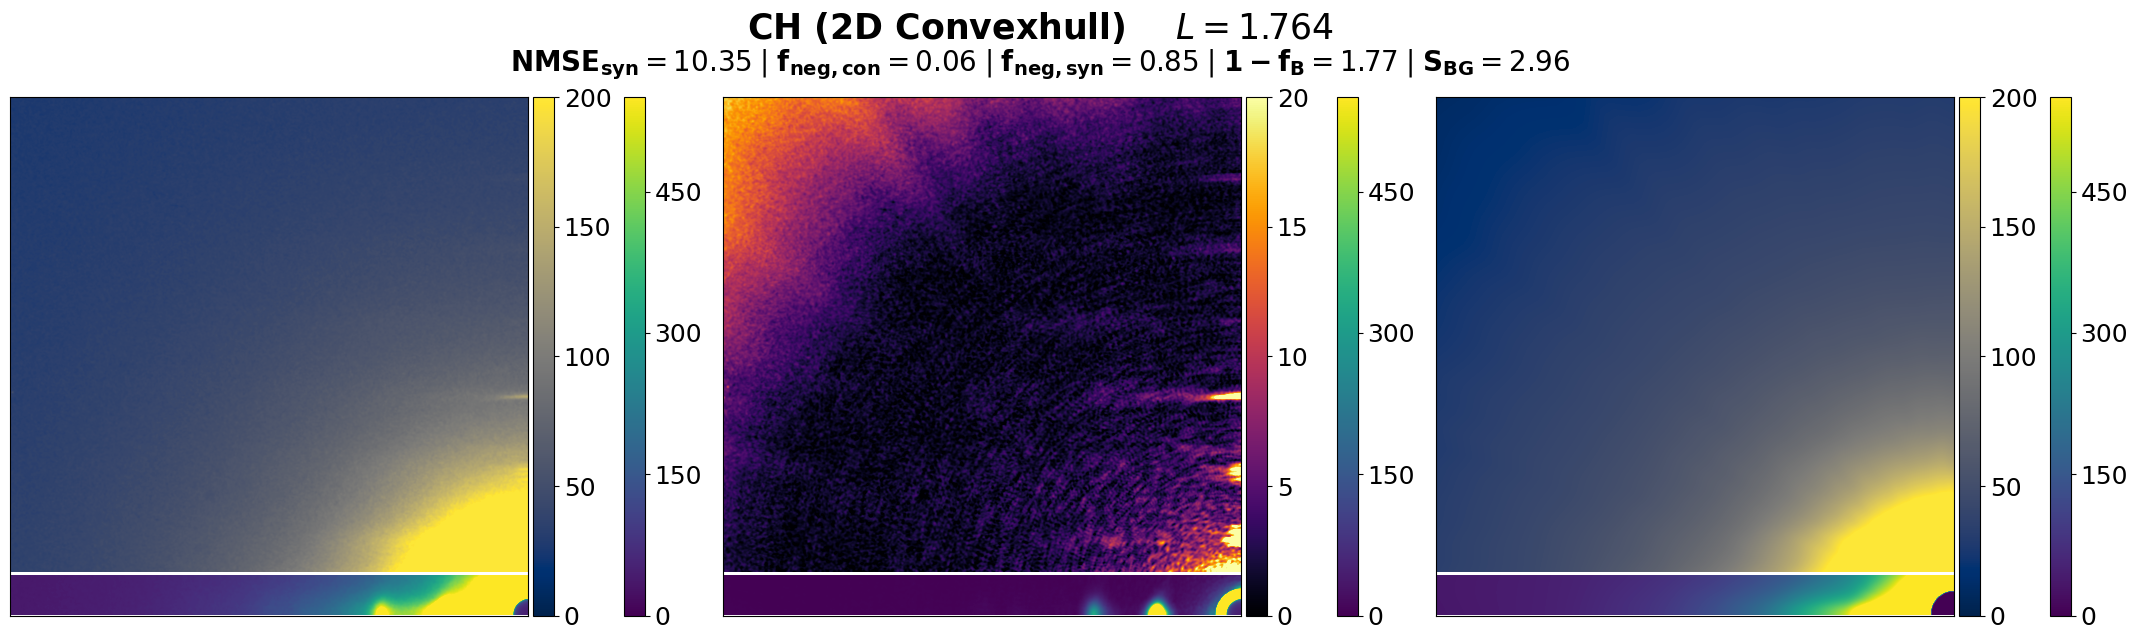
\includegraphics[width=0.95\linewidth]{figs/Fig4_ch_example_Jani_1_zoomed_v3.png}
\caption{Example of the equatorial streak background subtraction using the RCH method. Left to right: original image, background-subtracted image with RCH, backgrounds. The equatorial streak is removed but radial streak artifacts are introduced at higher scattering angles. Two scales are used for visualization due to the large intensity differences betweenthe equatorial streak and the rest of the pattern.}
\label{fig:ch_example}
\end{figure}

Additionally to the previosuly described framework, we propose a complementary iterative two-stage procedure to jointly model the anisotropic equatorial streak and the surrounding general background, extending subtraction to the whole pattern. Full methodological details are given in Section~\ref{sec:two_stage}. 
% The selection of methods and datasets is described in Section~\ref{sec:experimental_design}.
% The datasets used throughout are summarized in Table~\ref{tab:datasets}.
% (Section~\ref{sec:two_stage})



%%%%%%%%%%%%%%%%%%%%%%%%%%%%%%%%%%%%%%%%%%
\section{Results}

This section summarizes the performance of the framework in optimizing the background subtraction methods. We aim to evaluate whether an optimal solution to the problem of background subtraction can be identified given the lack of ground-truth background. The goal is not to identify a single universally optimal method, but to illustrate how the framework provides a consistent, quantitative basis for comparing methods and analyzing their behavior across diverse datasets. Methods may be compared using the aggregate loss function and its constituent metrics, with lower values indicating improved background removal, reduced artifacts, and better preservation of faint diffraction features.

We first evaluate representative visual examples. Then, we demonstrate convergence and consistency of the outputs of the optimization framework, followed by  a quantitative comparison of the optimized methods across datasets and analysis of optimized parameters. Finally, we evaluate the iterative two-stage refinement, a combined approach for whole-pattern background subtraction, including the equatorial streak, both visually and using the same standardized metrics, reported separately for the equatorial region and the general region.

\subsection{Visual Correspondence with Quantitative Metrics}
\label{sec:visual_correspondence}

Figure~\ref{fig:visual_no_eq} illustrates representative examples corresponding to low-loss background subtraction outcomes for images from 3 different datasets. In the low-loss examples, diffuse background is effectively removed while diffraction features are preserved and the residual baseline remains smooth. Appendix Figure \ref{fig:example_1img_all_bg} show an example of background subtraction outcomes for different methods applied to the same pattern, allowing to appreciate the differences in methods and performance. In the higher-loss examples, the methods exhibit either incomplete background removal, with elevated residual intensity between layer lines or excessive background removal. These visual differences correspond to the quantitative loss values, indicating that the evaluation metrics reflect perceptually meaningful aspects of background subtraction quality.

\begin{figure}[h]
\centering
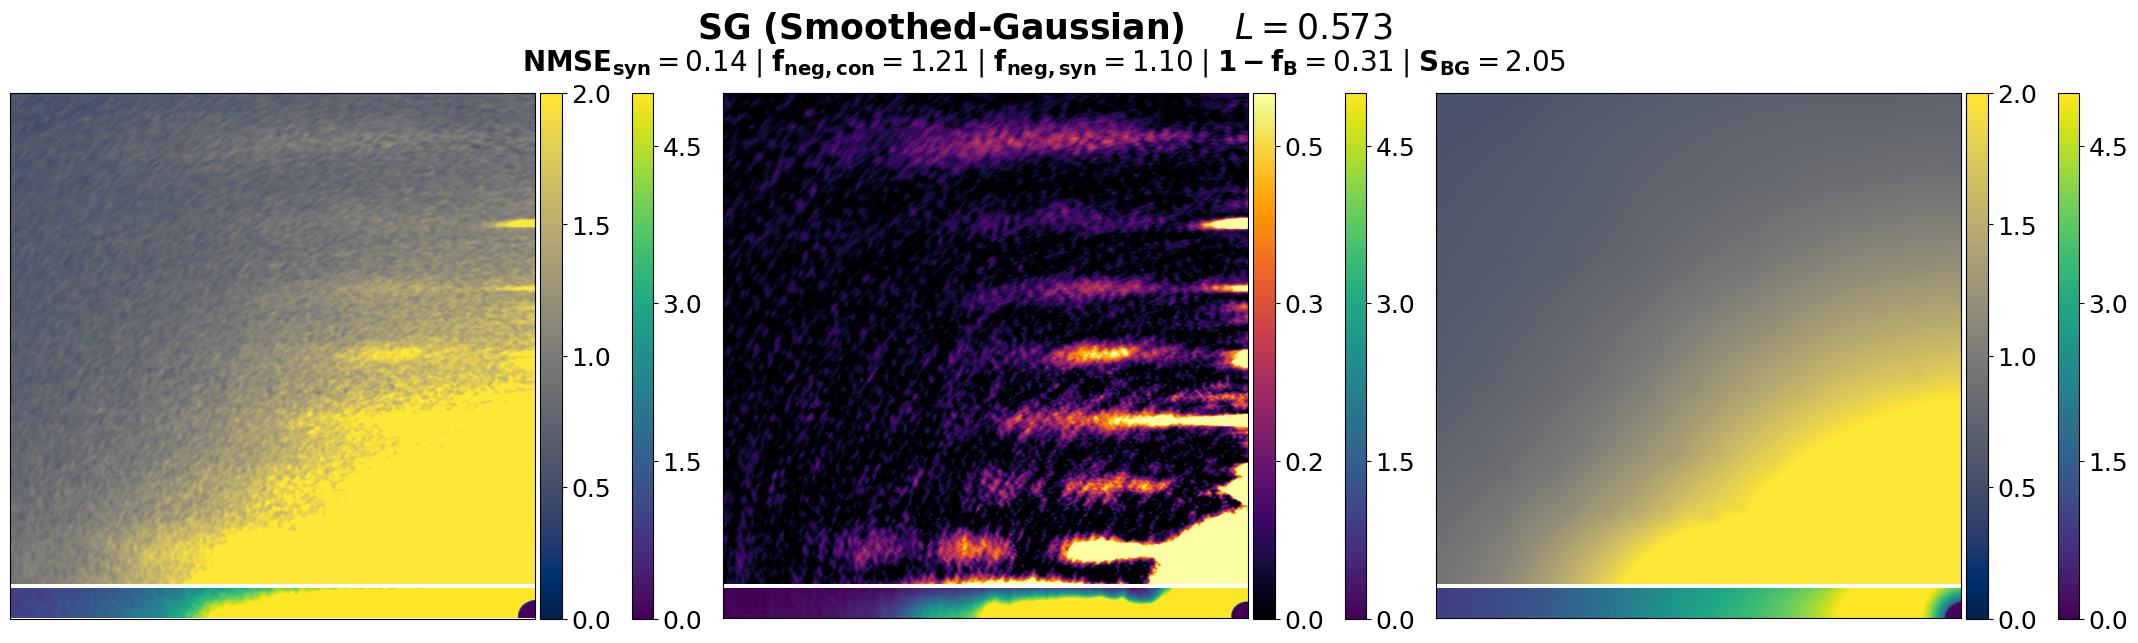
\includegraphics[width=0.58\linewidth]{figs/Fig9_visual_no_eq_sg_Granzier_21_v3.png}
\hspace{0.01\linewidth}
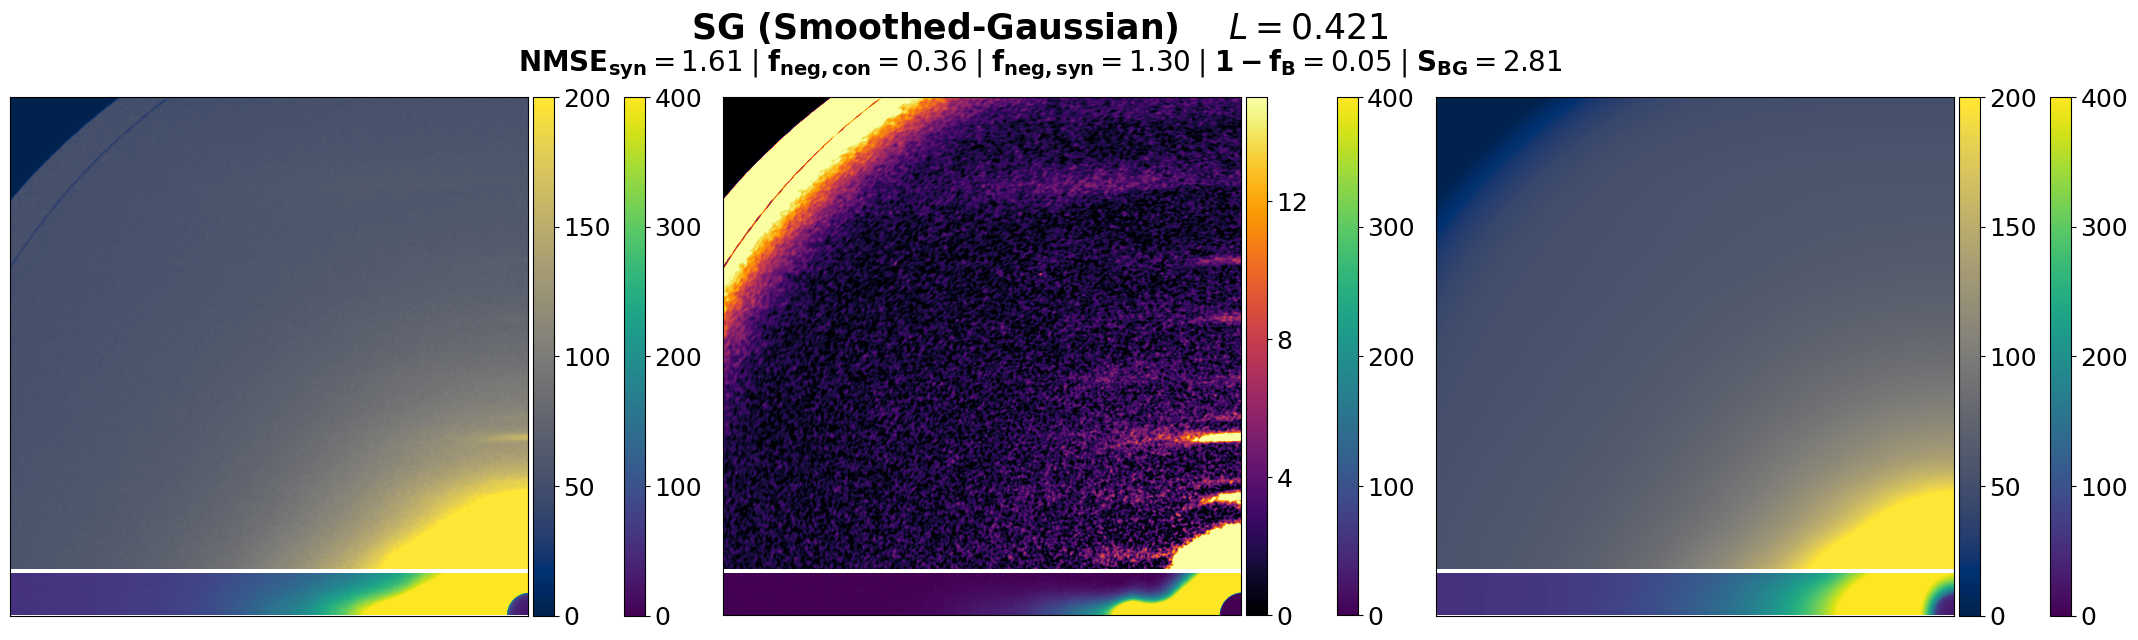
\includegraphics[width=0.58\linewidth]{figs/Fig9_visual_no_eq_MPLL_20_v3.png}
\hspace{0.01\linewidth}
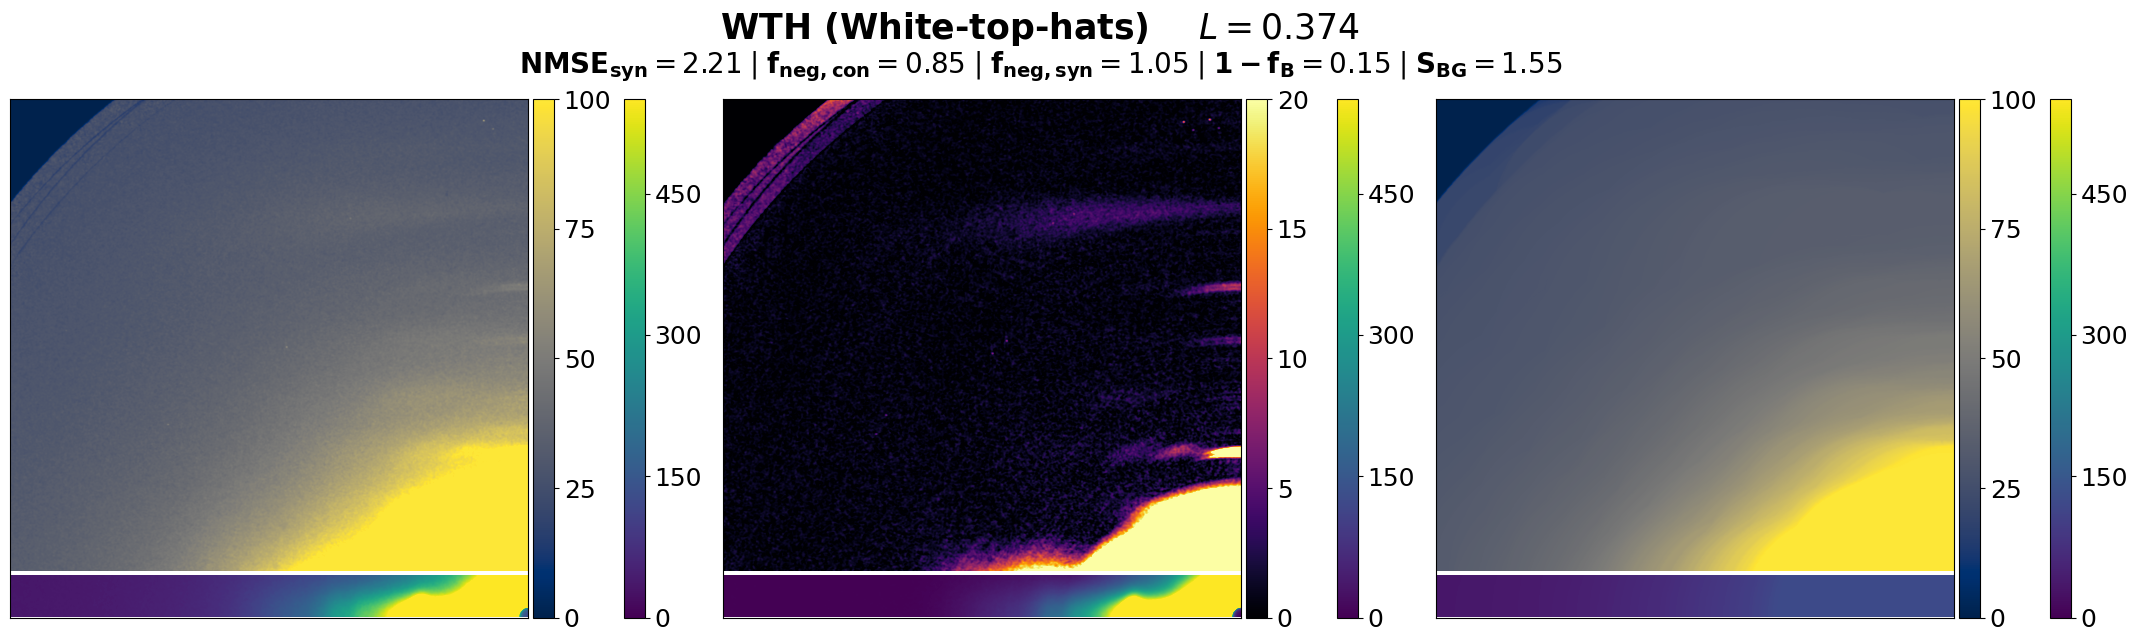
\includegraphics[width=0.58\linewidth]{figs/Fig9_visual_no_eq_Jani_21_v3.png}
\caption{Examples of successful background subtraction outcomes for different images. Each row is a different pattern from three datasets. Left to right: original image before subtraction, background-sutracted pattern, and background. Two scales are used for visualization due to high intensity differences between the background, the equatorial streak and the rest of the pattern. The selected method and paramemeters effectively remove the background while preserving faint features for both high intensity shown in the top two rows and low intensity pattern in the bottom row.}
\label{fig:visual_no_eq}
\end{figure}

\subsection{Convergence and Consistency of Optimization}
\label{sec:convergence}

The optimization framework demonstrates robust convergence and consistency across different datasets. Figure ~\ref{fig:consistency_bgsum} shows the low average background intensity dispersion per dataset, which is expected to be consistent within datasets, since patterns are taken with the same exposure time. The caption shows that although the best-performing method varies with dataset, WTH is ranked first in most datasets, with the remaining datasets split among G-ILPF, RW, and AVG. Optimization traces reflect that the optimization process is stable and makes choices based on the assigned weights. All the methods converge to similar loss values and the stopping criteria is either no loss improvement or very small change.

% Figure~\ref{fig:consistency_ranking} reflects low average loss dispersion within datasets for all but three datasets, which suggests the need for image-subset tuning. It also shows that although the best-performing method varies with dataset, WTH is ranked first in 6 of the 11 datasets, with the remaining datasets split among G-ILPF, RW, and AVG.

% \begin{figure}[h]
% \centering
% 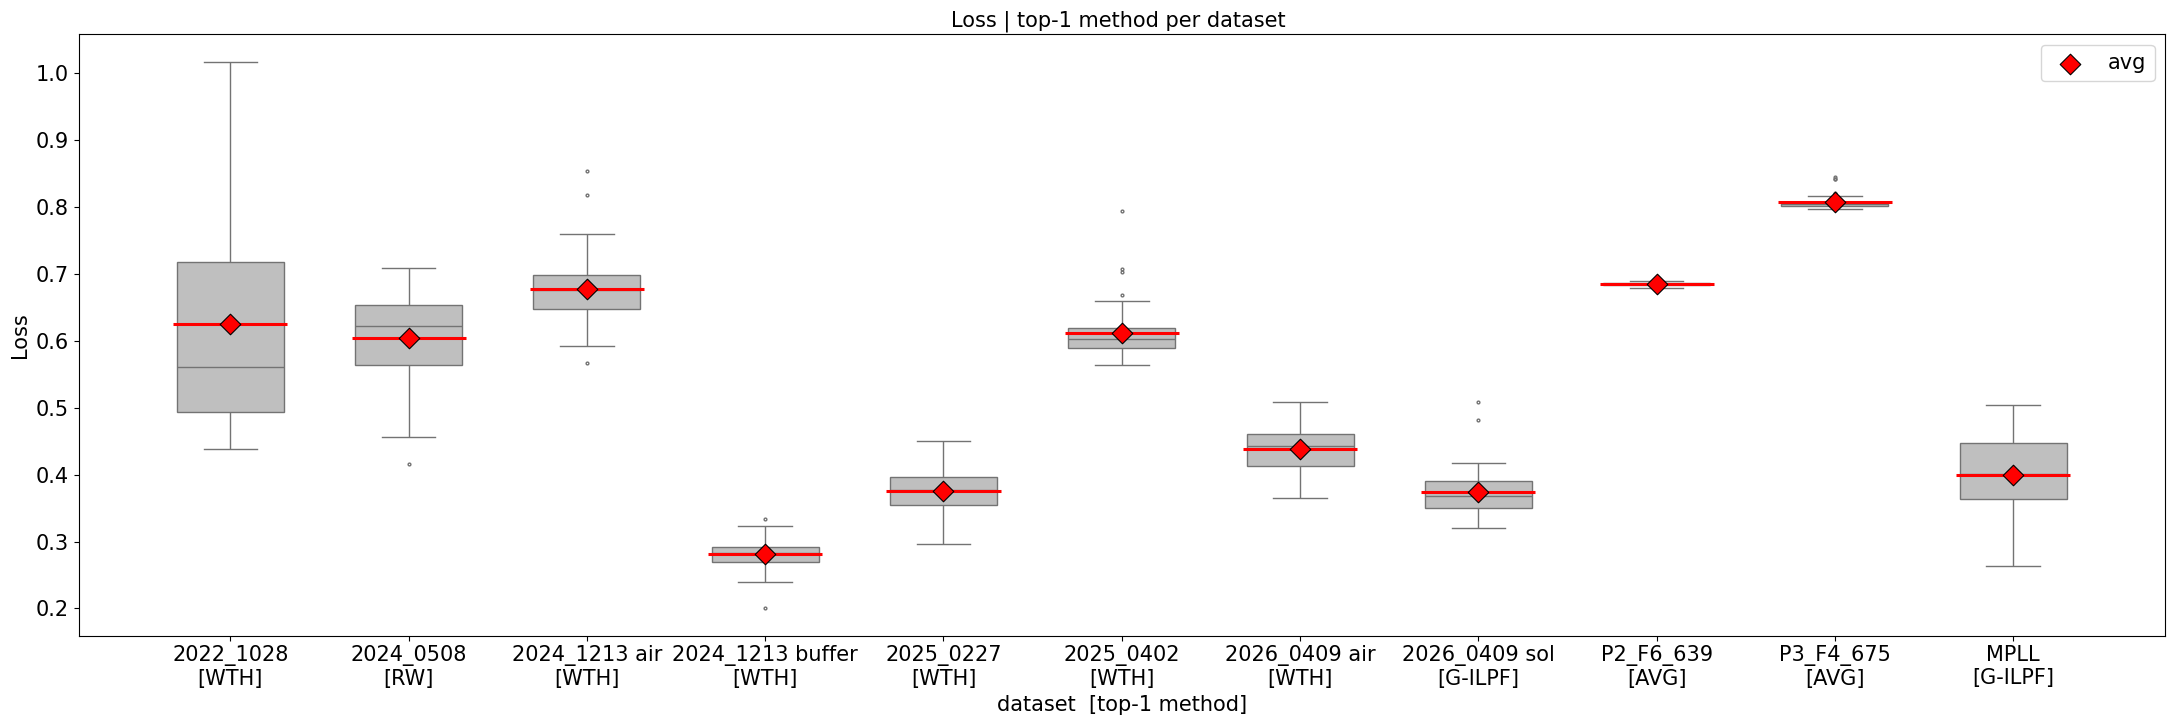
\includegraphics[width=0.95\linewidth]{figs/Fig7_consistency_ranking.png}
% \caption{Consistency of optimization results wihtin datasets. Distribution of best-per-image loss by dataset. Most datasets show low dispersion, except for three datasets, suggesting the need for image-subset tuning. Best method per dataset is shown in brackets.}
% \label{fig:consistency_ranking}
% \end{figure}

\begin{figure}[h]
\centering
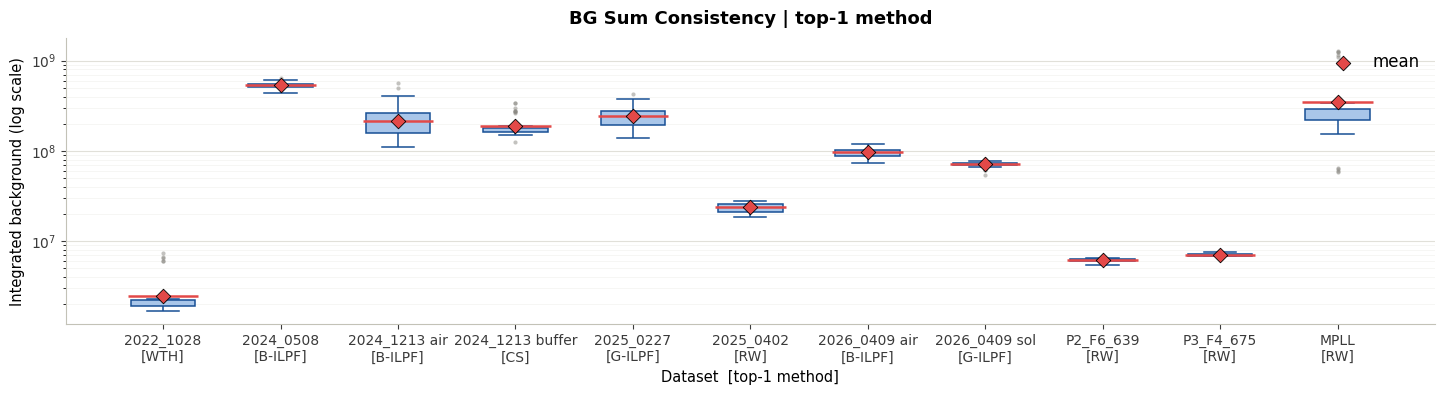
\includegraphics[width=1.0\linewidth]{figs/Fig8_consistency_bgsum_v2.png}
\caption{Consistency of optimization results within datasets. Distribution of average background intensity per dataset. The background intensity is consistent within datasets. Best method per dataset is shown in brackets.}
\label{fig:consistency_bgsum}
\end{figure}

\subsection{Quantitative Comparison of Methods}
\label{sec:quant_comparison}

Table~\ref{tab:method_performance_new} reports the aggregate loss and individual metric values for each background subtraction method, averaged over all evaluated datasets. Lower values indicate better performance for all reported metrics. Overall, the white-top-hat approach produces the lowest average loss values in this study. The iterative low pass filtering approaches also perform competitively, with different trade-offs across individual metrics. The AVG baseline, which is calculated as the average of the non-masked regions, shows that CS and RCH methods do not perform well due to the synthetic data distortion and roughness of the background. Since the equator streak is masked out, the evaluation focuses on high angle background, where RCH method does not perform well due to the artifacts introduced at high angles. The average baseline confirms that spatially structured background modeling is essential for reliable subtraction, since for AVG the fraction of the baseline residuals is high, which is the main driver for backgroundsubtraction. The AVG method is expected to perform poorly on patterns with high background intensity due to oversubtraction; however, it might perform competitively on patterns with low background intensity at high angles, for example in the datasets P2\_F6\_639 and P3\_F4\_675, where there is very little background intensity. The individual metric values reveal trade-offs between methods. For example, low-pass filtering approaches and white-top-hat generally achieve low synthetic feature oversubtraction and low synthetic feature distortion, indicating good preservation of faint injected features, while the circularly symmetric method tends to oversubtract synthetic signal. No single metric dominates performance across all methods (see Appendix Figure~\ref{fig:example_1img_metrics}), underscoring the need for a composite evaluation criterion.

\begin{table}[h]
\caption{Comparison of background subtraction methods across all evaluated images. Values are reported as mean $\pm$ st.dev. to emphasize the variability of performance across datasets rather than absolute rankings. Lower values indicate better performance for each metric. The AVG method is a constant-background baseline included as a sanity check and is not expected to perform well on spatially varying backgrounds; it might however perform well on pattern with low background intensity. Best values are highlighted in bold and second-best in underline.}
\label{tab:method_performance_new}
\centering
\small
\setlength{\tabcolsep}{3pt}
\renewcommand{\arraystretch}{1.1}
\begin{tabular}{@{}lcccccc@{}}
\toprule
\textbf{Method} & $\mathbf{Loss}$ & $\mathbf{NMSE}_{\mathbf{syn}}$ & $\mathbf{f}_{\mathbf{neg,con}}$ & $\mathbf{f}_{\mathbf{neg,syn}}$ & $\mathbf{1-f_B}$ & $\mathbf{S}_{\mathbf{BG}}$ \\
\midrule
AVG & 0.73 $\pm$ 0.12 & \textbf{0.92 $\pm$ 9.79} & 4.02 $\pm$ 0.11 & 1.34 $\pm$ 0.09 & 0.56 $\pm$ 0.08 & \textbf{0.00 $\pm$ 0.00} \\
WTH & \textbf{0.58 $\pm$ 0.23} & 2.81 $\pm$ 3.57 & 1.12 $\pm$ 0.66 & \underline{0.98 $\pm$ 0.20} & 0.34 $\pm$ 0.25 & \underline{1.81 $\pm$ 0.71} \\

G-ILPF & \underline{0.61 $\pm$ 0.24} & 1.50 $\pm$ 1.65 & 1.10 $\pm$ 0.57 & 1.18 $\pm$ 0.23 & 0.35 $\pm$ 0.30 & 2.06 $\pm$ 0.80 \\
B-ILPF & 0.67 $\pm$ 0.20 & 3.00 $\pm$ 3.50 & 1.37 $\pm$ 0.71 & 1.25 $\pm$ 0.20 & \textbf{0.25 $\pm$ 0.21} & 3.19 $\pm$ 1.46 \\
CS & 1.01 $\pm$ 0.54 & 2.11 $\pm$ 10.89 & \underline{0.86 $\pm$ 0.73} & 1.02 $\pm$ 0.37 & 0.80 $\pm$ 0.73 & 2.82 $\pm$ 1.47 \\
RCH & 1.78 $\pm$ 0.45 & 13.05 $\pm$ 25.89 & \textbf{0.10 $\pm$ 0.08} & \textbf{0.80 $\pm$ 0.26} & 1.55 $\pm$ 0.71 & 3.80 $\pm$ 1.69 \\
RW & 0.71 $\pm$ 0.27 & \underline{1.02 $\pm$ 1.37} & 1.77 $\pm$ 0.55 & 1.00 $\pm$ 0.31 & \underline{0.27 $\pm$ 0.21}  & 3.56 $\pm$ 1.31  \\

\bottomrule
\end{tabular}
\end{table}

\subsection{Optimized Parameter Variability}
\label{sec:param_variability}

Optimized parameter variability for each method is summarized in Table~\ref{tab:summary_total_variability}. The fitted coefficients show considerable variability across all images. This variability reflects differences in background structure arising from experimental conditions, detector characteristics, and sample preparation. For several methods, the large variability across all images indicates that optimal parameters depend strongly on dataset-specific characteristics. Within datasets the variability is significantly lower; however, it is still considerable. This observation suggests that further performance gains may be achievable by clustering diffraction patterns based on background properties and selecting method parameters accordingly, rather than using a single global configuration. Part of this residual spread may reflect parameter degeneracy rather than genuinely distinct optimal solution: the low within-dataset dispersion in loss and background intensity indicates that different coefficient combinations can produce comparably good subtraction outcomes for the same dataset. Under this interpretation, the optimizer may converge to different but similarly effective parameter sets depending on initialization or image-specific noise, rather than any single configuration being uniquely optimal. Overall, the large spread in optimized coefficients demonstrates that parameter values are not stable across datasets, reinforcing the need for image-specific or dataset-adaptive background subtraction strategies.

\begin{table}[h]
\centering
\footnotesize
\caption{Coefficient variability (st.dev./mean) across images and datasets (mean $\pm$ st.dev). Even though variability is lower within datasets, adaptive dataset-specific and image-specific tuning should be considered.}
\label{tab:summary_total_variability}
\begin{tabular}{llccc}
\toprule
Method & Parameter & Across-images CV & Between-datasets CV & Difference \\
\midrule

RCH & degree & 0.00 & 0.00 & 0.00 \\
CS & radial bin & 3.13 & 0.57 & -2.56 \\
CS & smooth & 2.73 & 0.99 & -1.75 \\
CS & cirmin & 2.17 & 2.08 & -0.09 \\
CS & cirmax & 1.21 & 0.60 & -0.61 \\
RW & cirmin & 2.21 & 3.45 & 1.24 \\
RW & window sep$_x$ & 1.11 & 1.20 & 0.08 \\
RW & window sep$_y$ & 1.09 & 1.02 & -0.07 \\
RW & tension & 0.88 & 0.83 & -0.06 \\
RW & window size$_x$ & 0.73 & 0.62 & -0.12 \\
RW & window size$_y$ & 0.55 & 0.40 & -0.15 \\
RW & cirmax & 0.41 & 0.34 & -0.07 \\
% RW & smooth & -- & -- & -- \\
B-ILPF & boxcar$_y$ & 1.13 & 0.59 & -0.54 \\
B-ILPF & boxcar$_x$ & 1.08 & 0.66 & -0.42 \\
B-ILPF & cycles & 0.61 & 0.37 & -0.24 \\
G-ILPF & cycles & 0.68 & 0.31 & -0.37 \\
G-ILPF & FWHM & 0.49 & 0.26 & -0.23 \\
WTH & tophat & 0.33 & 0.21 & -0.12 \\
\midrule
Mean &  & 1.14 & 0.81 & -0.33 \\

\bottomrule
\end{tabular}
\end{table}


\subsection{Evaluation of Iterative Two-Stage Background Subtraction}
\label{sec:two_stage_eval}

The iterative two-stage pipeline for fitting the equtatorial steak $E$ and general background $G$ produces a single residual, $\mathrm{img} - E - G$, covering the entire pattern. We evaluate the performance of this approach by analyzing the residual in both the general high-angle region (same as in the previous section) and the equatorial region. Reporting a single full-pattern number would obscure how the two fitted components contribute to the result in each region, since the low angle equatorial and high angle general regions require different masking. For the equatorial region evaluation, the aggregate loss is computed with a modified set of weights relative to Section~\ref{sec:quant_comparison}: the smoothness term is dropped ($\lambda_1 = 0$), since in the equatorial region, the background is expected to be steep. Relative to the default weighting used there ($[\lambda_1,\ldots,\lambda_5] = [0.1, 0.05, 0.05, 0.01, 0.8]$), the weight removed from smoothness is redistributed evenly to the two oversubtraction terms, $f_{\mathrm{neg,con}}$ and $f_{\mathrm{neg,syn}}$, giving $[\lambda_1, \lambda_2, \lambda_3, \lambda_4, \lambda_5] = [0, 0.1, 0.1, 0.01, 0.8]$. The evaluation of the general background region is performed in the same way as in the previous section.

A key advantage of the iterative two-stage approach is its ability to perform background subtraction on the whole pattern, ensuring that the equatorial streak and the general background are both properly accounted for. Representative examples of the equatorial streak fitting and the optimized general background produced by the iterative pipeline are shown in Figure~\ref{fig:visual_eq}. Due to the large intensity differences between the background, the equatorial streak and the rest of the pattern, multiple scales are used for visualization. 

\subsubsection{General Background Comparison.}

Table~\ref{tab:two_stage_full} reports the resulting metrics over the same region as in the previous analysis (beam center, detector edges and the equator region masked) for the radial convex hull baseline (RCH), for the iterative two-stage fit alone (Fit), and for the iterative fit combined with each framework method applied to the residual general background (Fit+G-ILPF, Fit+WTH, Fit+B-ILPF, Fit+RW).

\begin{table}[H]
\caption{Cross-dataset comparison of background subtraction methods over the general background region of the pattern (equator masked). RCH is the radial convex hull baseline from Table~\ref{tab:algorithms}; Fit is the iterative two-stage equatorial-plus-general fit (Section~\ref{sec:two_stage}) without further refinement; the remaining rows combine that fit with each framework method applied to the residual general background. The aggregate loss drops the smoothness term. Values are mean $\pm$ st.dev.\ across images. Best values are highlighted in bold and second-best in underline; tied values are underlined jointly.}
\label{tab:two_stage_full}
\centering
\small
\setlength{\tabcolsep}{3pt}
\renewcommand{\arraystretch}{1.1}
\begin{tabular}{@{}lcccccc@{}}
\toprule
\textbf{Method} & $\mathbf{NMSE}_{\mathbf{syn}}$ & $\mathbf{f}_{\mathbf{neg,syn}}$ & $\mathbf{1-f_B}$ & $\mathbf{f}_{\mathbf{neg,con}}$ & $\mathbf{S}_{\mathbf{BG}}$ & \textbf{Loss} \\
\midrule
RCH & 13.05 $\pm$ 25.89 & \underline{0.80 $\pm$ 0.26} & 1.55 $\pm$ 0.71 & \underline{0.10 $\pm$ 0.08} & 3.80 $\pm$ 1.69 & 1.79 $\pm$ 0.46 \\
Fit & \textbf{0.00 $\pm$ 0.00} & \textbf{0.00 $\pm$ 0.00} & 2.55 $\pm$ 0.57 & \textbf{0.03 $\pm$ 0.06} & \textbf{3.26 $\pm$ 1.68} & 2.36 $\pm$ 0.42 \\
Fit+G-ILPF & 0.96 $\pm$ 1.38 & 1.17 $\pm$ 0.18 & \underline{1.38 $\pm$ 0.70} & 0.96 $\pm$ 0.45 & \underline{3.39 $\pm$ 1.51} & \underline{1.55 $\pm$ 0.56} \\
Fit+WTH & 1.07 $\pm$ 1.45 & \underline{0.80 $\pm$ 0.25} & 1.41 $\pm$ 0.72 & 0.92 $\pm$ 0.52 & 3.54 $\pm$ 1.40 & 1.57 $\pm$ 0.55 \\
Fit+B-ILPF & 1.01 $\pm$ 1.39 & 1.13 $\pm$ 0.22 & 1.39 $\pm$ 0.70 & 1.02 $\pm$ 0.44 & 3.51 $\pm$ 1.46 & 1.57 $\pm$ 0.56 \\
Fit+RW & \underline{0.35 $\pm$ 0.42} & 1.17 $\pm$ 0.22 & \textbf{0.85 $\pm$ 0.44} & 2.27 $\pm$ 0.59 & 3.50 $\pm$ 1.51 & \textbf{1.20 $\pm$ 0.38} \\
\bottomrule
\end{tabular}
\end{table}

\begin{figure}[h]
\centering
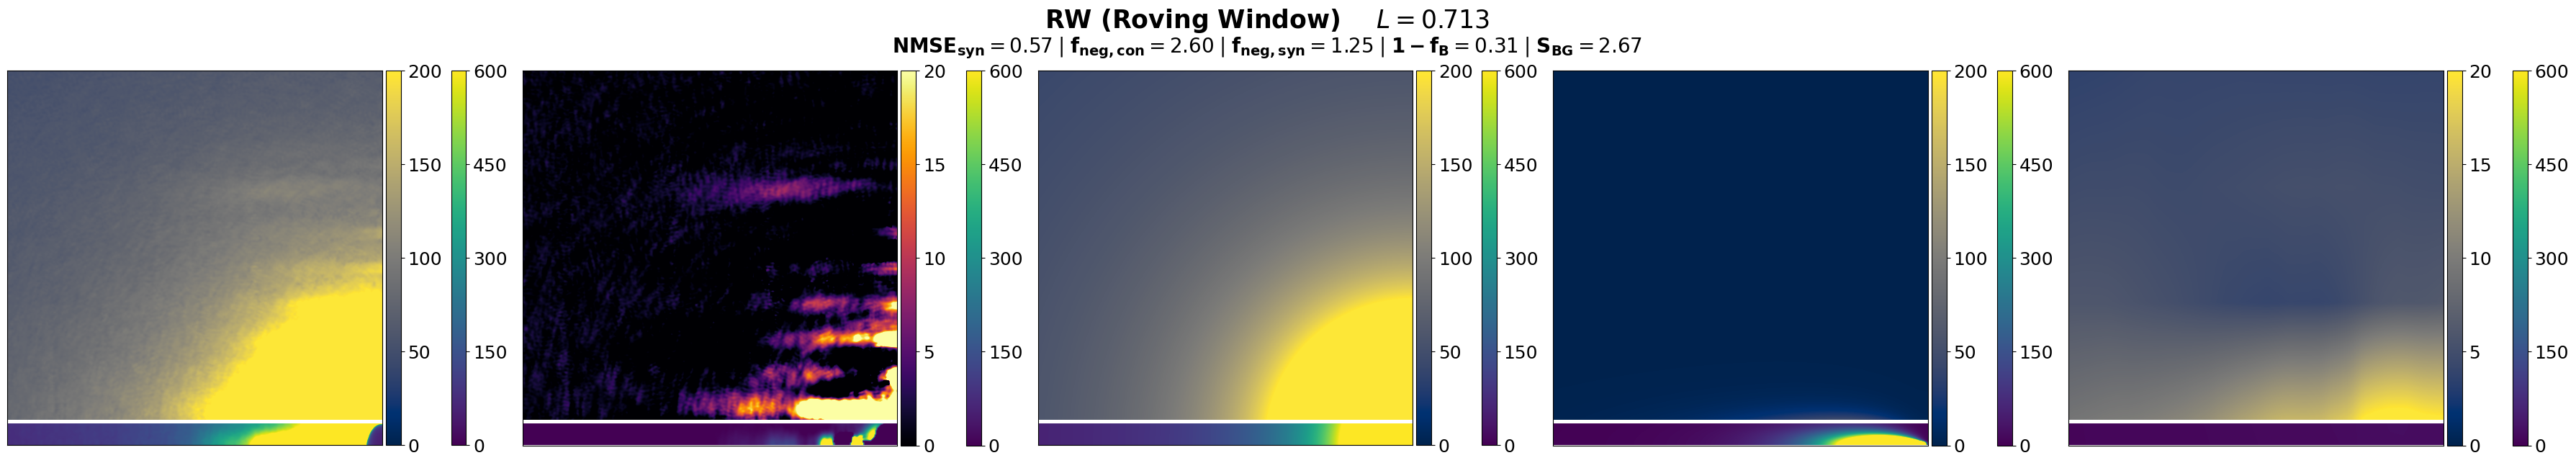
\includegraphics[width=0.95\linewidth]{figs/Fig11_visual_eq_Weikang_4_v3.png}
\hspace{0.01\linewidth}
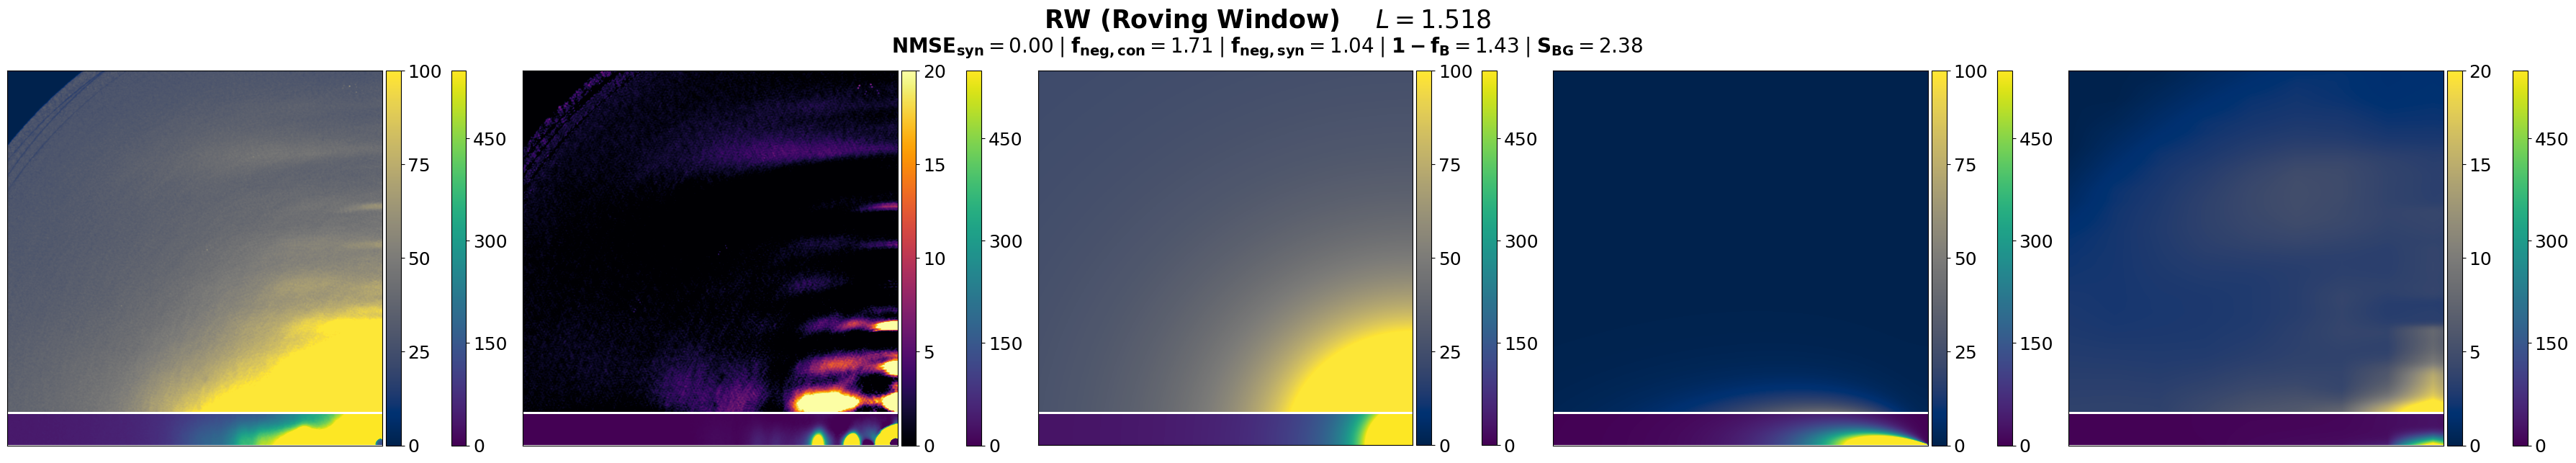
\includegraphics[width=0.95\linewidth]{figs/Fig11_visual_eq_Jani_21_v3.png}
\hspace{0.01\linewidth}
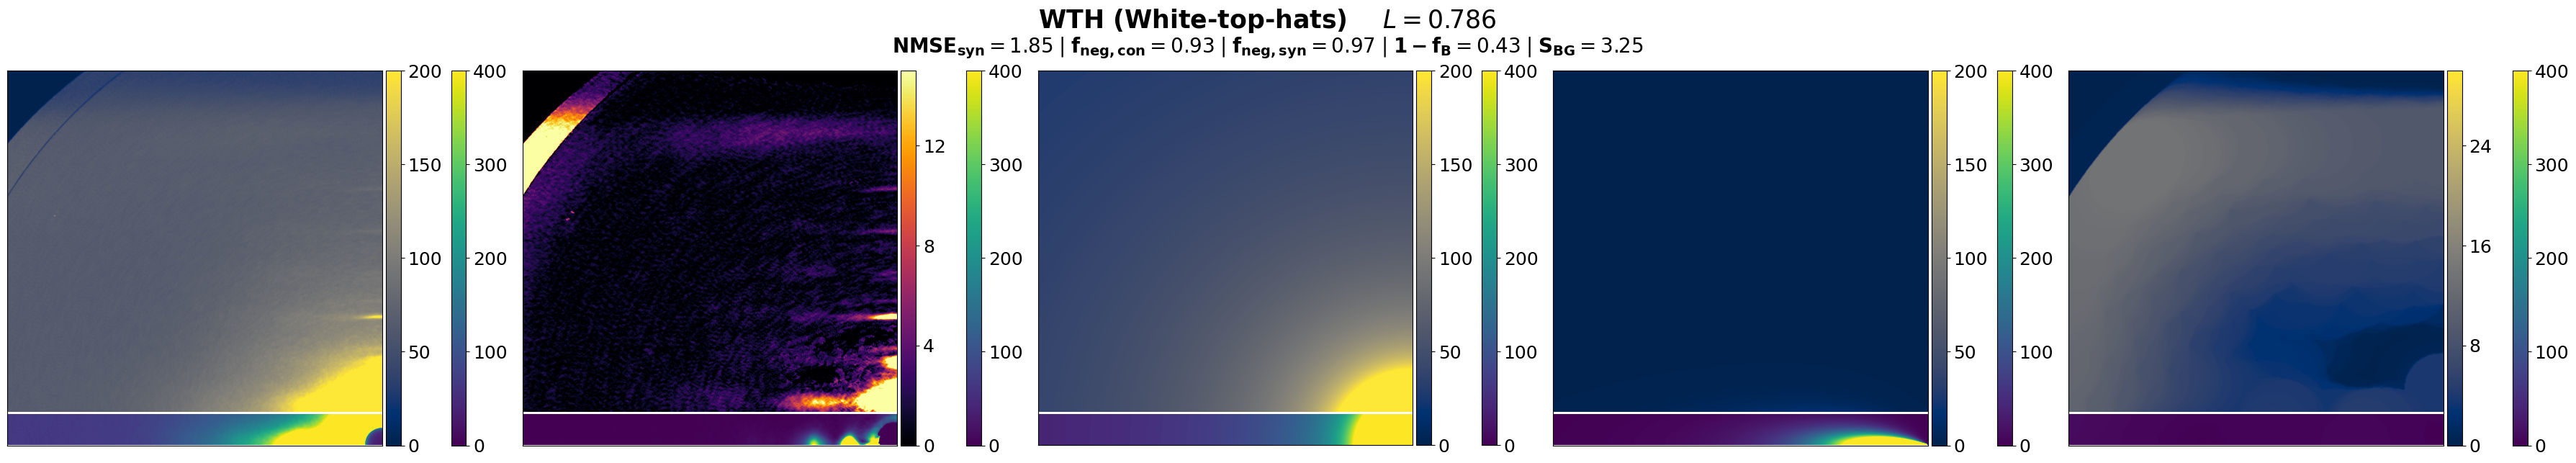
\includegraphics[width=0.95\linewidth]{figs/Fig11_visual_eq_MPLL_2_v3.png}
\hspace{0.01\linewidth}
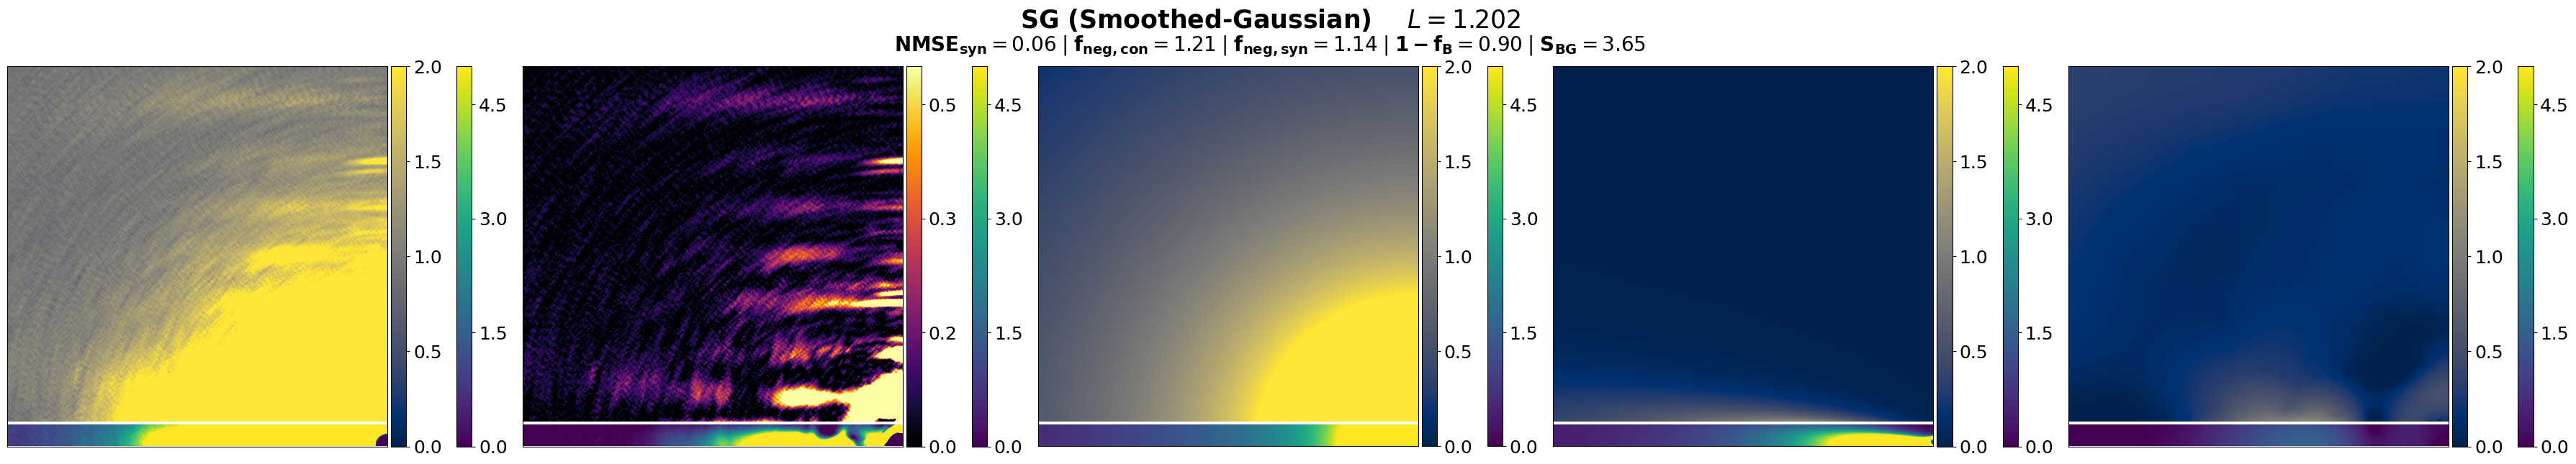
\includegraphics[width=0.95\linewidth]{figs/Fig11_visual_eq_Granzier_4_v3.png}
\caption{Examples of successful background subtraction outcomes for different patterns with fitted equatorial streaks. Each row is a different pattern from four datasets. Left to right: original image before subtraction, background-sutracted pattern, fitted general background, fitted equatorial streak, and the non-parametric background for the remaining residual. Two scales are used for visualization due to high intensity differences between the equatorial streak and the rest of the pattern. The equatorial streak is removed and the smooth background is removed from the pattern.}
\label{fig:visual_eq}
\end{figure}


The iterative fit alone results in zero $\mathrm{NMSE}_{\mathrm{syn}}$ and $f_{\mathrm{neg,syn}}$, reflecting negligible local oversubtraction, and produces the smoothest background, but as expected by design leaves the highest residual baseline. Applying non-parametric methods using the framework to the remaining residual background reduces the loss substantially: Fit+RW reaches the lowest loss, and all four combinations outperform the RCH baseline. This confirms that the iterative fit removes the dominant, anisotropic equatorial streak and most of the general background, but a residual slowly varying component remains that a non-parametric framework method can remove on top of the fit, producing a cleaner background than either RCH alone or the iterative fit alone.

\subsubsection{Equatorial-Region Comparison}
To isolate the contribution of the equatorial-streak fit itself, Table~\ref{tab:two_stage_equator} reports the same set of methods restricted to the equator mask alone (Section~\ref{sec:masking}), using the aggregate loss with the smoothness term dropped.


\begin{table}[t]
\caption{Comparison of background subtraction methods restricted to the equatorial region (Section~\ref{sec:masking}). Method definitions, weights, and column conventions are as in Table~\ref{tab:two_stage_full}; metrics here are computed using the equator mask only. Best values are highlighted in bold and second-best in underline; tied values are underlined jointly. Loss doesn't include the smoothness term.}
\label{tab:two_stage_equator}
\centering
\small
\setlength{\tabcolsep}{3pt}
\renewcommand{\arraystretch}{1.1}
\begin{tabular}{@{}lcccccc@{}}
\toprule
\textbf{Method} & $\mathbf{NMSE}_{\mathbf{syn}}$ & $\mathbf{f}_{\mathbf{neg,syn}}$ & $\mathbf{1-f_B}$ & $\mathbf{f}_{\mathbf{neg,con}}$ & $\mathbf{S}_{\mathbf{BG}}$ & \textbf{Loss} \\
\midrule
RCH & 69.71 $\pm$ 504.53 & \underline{0.72 $\pm$ 0.37} & \underline{1.67 $\pm$ 0.50} & \underline{0.04 $\pm$ 0.03} & \textbf{18.11 $\pm$ 9.55} & 2.11 $\pm$ 5.02 \\
Fit & \textbf{0.00 $\pm$ 0.00} & \textbf{0.00 $\pm$ 0.00} & 2.58 $\pm$ 0.44 & \textbf{0.03 $\pm$ 0.12} & 26.86 $\pm$ 26.47 & 2.07 $\pm$ 0.35 \\
Fit+G-ILPF & 2.12 $\pm$ 6.20 & 1.17 $\pm$ 0.22 & 1.86 $\pm$ 0.50 & 0.68 $\pm$ 0.30 & 26.93 $\pm$ 26.16 & 1.69 $\pm$ 0.37 \\
Fit+WTH & \underline{0.99 $\pm$ 4.05} & 0.75 $\pm$ 0.28 & 1.84 $\pm$ 0.50 & 0.64 $\pm$ 0.31 & \underline{26.77 $\pm$ 26.23} & \underline{1.61 $\pm$ 0.37} \\
Fit+B-ILPF & 2.14 $\pm$ 5.64 & 1.10 $\pm$ 0.25 & 1.93 $\pm$ 0.54 & 0.69 $\pm$ 0.36 & 26.98 $\pm$ 26.10 & 1.74 $\pm$ 0.39 \\
Fit+RW & 3.40 $\pm$ 72.05 & 1.19 $\pm$ 0.26 & \textbf{1.43 $\pm$ 0.44} & 1.78 $\pm$ 0.61 & 27.22 $\pm$ 26.04 & \textbf{1.48 $\pm$ 0.79} \\
\bottomrule
\end{tabular}
\end{table}

Within the equatorial region, the iterative fit alone already achieves a lower loss than the RCH baseline, and does so with a far lower variation, indicating that RCH's behavior in the equatorial region is variable across images whereas the parametric fit is consistently stable. As in the full-pattern comparison, applying a framework method to the residual after the equatorial fit further reduces the loss, with Fit+RW showing the highest variability among the combinations in this region while the other three are the most consistent.

%%%%%%%%%%%%%%%%%%%%%%%%%%%%%%%%%%%%%%%%%%
\section{Discussion}
\label{sec:discussion}

Taken together, these results demonstrate that the proposed optimization framework provides a consistent and objective basis for comparing background subtraction methods across diverse datasets. Since subtraction quality is evaluated by defined, physically motivated metrics rather than by visual inspection, methods that make different structural assumptions can be placed on a common scale, and the aggregate loss correlates with the expert visual assessment of the patterns. This addresses the central limitation of current approach, in which operator intervention and subjective assessment make results difficult to reproduce and compare.

No single background subtraction method dominates across all metrics or all datasets. The white top-hat filter has the lowest average loss; however, the iterative low-pass filters and the roving window method are competitive. No individual metric is sufficient to rank methods (Appendix Figure~\ref{fig:example_1img_metrics}), which is the core justification for a composite loss: the metrics encode competing aspects that must be balanced rather than optimized in isolation.

The parametric and non-parametric approaches address complementary failure modes and are most effective in combination. The iterative two-stage fit removes the dominant, anisotropic equatorial streak and most of the general background with negligible oversubtraction, but by design leaves a residual baseline; applying a non-parametric framework method to that residual removes the remaining slowly varying component and yields the lowest loss, in both the general-background region and the equatorial region itself. The combination of the iterative fitting with the framework therefore allows background subtraction across the whole pattern, a significant improvement over existing approaches that typically operate only on specific regions of the pattern. This separation of background components will enable more accurate analysis of diffraction features across the entire pattern and could contribute to future studies of how background structure changes with experimental conditions, since the background itself may carry useful information.

The appropriate choice of background subtraction strategy still depends on the data analysis goal: for low angles only, the RCH method is often efficient, sufficient and robust; for layer lines and high angles, the equator may be masked and the optimization framework applied to the rest of the pattern; for background subtraction across the whole pattern, the iterative approach for the equatorial and general background fitting combined with the framework may be used.

Two limitations constrain how broadly these results generalize. First, optimized parameters vary substantially across datasets, and to a lesser extent within them (Table~\ref{tab:summary_total_variability}), so a single globally tuned parameter set is unlikely to be optimal; dataset- or image-specific tuning should be applied rather than fixed defaults. Part of the residual within-dataset spread appears to reflect parameter degeneracy rather than genuinely distinct optima, since different coefficient combinations can produce comparably low loss and background intensity. Second, the loss weights require operator judgment: the framework automates the parameter search within a method but not the choice of how strongly to penalize each failure mode for a given task, and some artifacts, such as faint negative excursions or subtle layer-line distortion, remain difficult to capture numerically. We therefore recommend a hybrid workflow: automated search combined with human verification on a small image subset, followed by weight adjustment and full-dataset optimization, rather than a fully unsupervised pipeline.

%%%%%%%%%%%%%%%%%%%%%%%%%%%%%%%%%%%%%%%%%%
\section{Materials and Methods}
\label{sec:approach}

This section describes the methodological framework used to evaluate and optimize background subtraction methods for muscle fiber diffraction patterns. We define qualitative objectives and quantitative metrics that capture physically meaningful properties of successful background removal. To enable objective validation in the absence of ground truth, synthetic diffraction features and region-specific masking are introduced. These metrics are then combined into an aggregate loss function that guides parameter optimization for each background subtraction method. Finally, we describe the study design, including algorithm variants and dataset selection.


\subsection{Evaluation Framework}
\label{sec:evaluation_framework}

The evaluation framework is designed to provide objective, physically meaningful criteria for assessing the quality of background subtraction in muscle fiber diffraction images. The framework uses quantitative metrics derived from physical considerations and qualitative expectations, which enables reproducible comparison across methods and parameter settings.

\subsubsection{Qualitative Objectives}

An ideal background-subtracted diffraction image should satisfy several qualitative criteria. True diffraction features should be preserved with minimal distortion and remain clearly distinguishable from the background. The subtraction process should not introduce non-physical artifacts, such as extended negative regions or patterns resembling diffraction features (e.g. layer lines or reflection peaks), which would indicate over-subtraction. Since intensity values are non-negative by definition, negative excursions should be minimized. In regions free of diffraction signal, the residual background should be smooth, near zero, and free of structured intensity variations. Finally, for images acquired under similar experimental conditions, background subtraction results and optimal parameters should be consistent across frames. These qualitative objectives motivate the following metrics in order to capture deviations from the described objectives in a reproducible way.

\subsubsection{Quantitative Metrics}

Several metrics operate directly on the background-subtracted image to assess artifact introduction, background smoothness, and residual baseline behavior. \textit{Oversubtraction} is assessed by measuring the fraction of negative-valued pixels that belong to spatially connected clusters larger than a specified minimum size (e.g.\ nine pixels). Random noise typically produces isolated negative pixels, whereas systematic oversubtraction produces spatially connected regions. This metric, denoted $f_{\mathrm{neg,con}}$, is ideally zero. \textit{Residual background level} is quantified using the fraction of pixels whose intensity lies within a specified threshold of zero, denoted $f_{B}$. This metric reflects how effectively structured background has been removed while preserving natural noise. The threshold is estimated from the average intensity near the edge of the diffraction pattern, where background scattering is expected to be minimal. \textit{Background smoothness} is quantified by measuring the average absolute intensity difference between adjacent rows in masked background regions. This smoothness metric, denoted $\mathrm{S}_{\mathrm{BG}}$, captures the presence of structured or oscillatory residual background. It is defined as
\begin{equation}
\mathrm{S}_{\mathrm{BG}} =
\frac{1}{N} \sum_i \left| I(y_i + 1) - I(y_i) \right|,
\end{equation}
where the summation is performed over rows within masked background regions to exclude known diffraction features. Smooth residual backgrounds produce low values of this metric.

\subsubsection{Validation Using Synthetic Structures}

Because experimental diffraction images do not provide ground-truth background, synthetic diffraction features are introduced to evaluate preservation of faint signals after background subtraction. These validation metrics focus on signal loss and oversubtraction behavior. \textit{Preservation of synthetic signal} is quantified using the normalized offset-invariant mean squared error between the background-subtracted image and a reference image containing only the injected synthetic features, denoted $\mathrm{NMSE}_{\mathrm{syn}}$. Ideally, this value is zero, indicating perfect preservation of synthetic signal. Although synthetic features are placed in regions known not to contain real diffraction features, partial overlap between synthetic and real structures may increase this metric. Offset is evaluated and subtracted from the pattern to avoid oversubtraction. This metric focuses specifically on the preservation of synthetic signal where the pattern contains positive values. \textit{Oversubtraction of synthetic features} is further assessed by measuring the fraction of negative-valued pixels remaining after synthetic signal subtraction, denoted $f_{\mathrm{neg,syn}}$. This metric emphasizes non-physical negative excursions introduced by background removal and is ideally zero. The quantitative metrics used in the evaluation framework are summarized in Table~\ref{tab:loss_terms}. 

\subsection{Sampling Framework for Assessing Detail Preservation}
\label{sec:sampling_framework}

This subsection describes synthetic signal design used to enable objective evaluation of background subtraction performance as well as region-specific masking to isolate background-dominated areas for metric calculation.

\subsubsection{Synthetic Signal Validation Design}

To address the central limitation in the lack of ground-truth, we inject synthetic diffraction features resembling real signal into the images prior to background subtraction as summarized in Algorithm~\ref{alg:synthetic_signal}. Preservation of these features after subtraction provides a controlled measure of signal loss and oversubtraction. Synthetic features are modeled using two-dimensional Gaussian functions elongated along the horizontal axis, a tractable approximation of the more complex shape of real diffraction features such as layer lines. The synthetic feature is defined as
\begin{equation}
G(x, y) = A \exp\!\left(
-\frac{(x-x_0)^2}{2\sigma_x^2}
-\frac{(y-y_0)^2}{2\sigma_y^2}
\right),
\end{equation}
where $A$ is the amplitude, $(x_0, y_0)$ is the feature center, and $\sigma_x$ and $\sigma_y$ are the standard deviations along the horizontal and vertical axes, respectively. This formulation corresponds to an axis-aligned Gaussian without rotational components. The shape parameters are selected automatically for each image to match the scale of real diffraction features. Based on observed correlations in experimental data, $\sigma_x$ and $\sigma_y$ are derived from the average FWHM of prominent reflections, specifically the $I_{1,0}$ equatorial peak and the M1 and M3 meridional reflections. Specifically,
\begin{equation}
\sigma_x = \frac{I_{1,0}}{5} \times \frac{1}{2\sqrt{2\ln2}}, 
\qquad
\sigma_y = \frac{\mathrm{M1}}{20} \times \frac{1}{2\sqrt{2\ln2}}.
\end{equation}
The radial decay of synthetic feature intensity follows a $1/r$ model, where $r$ is the distance from the pattern center. This choice reflects the scattering geometry of X-ray diffraction and approximates the Lorentz correction, which for equatorial and meridional reflections can be expressed as $L \propto 1/\sin 2\theta$~\citep{Buerger1940}. At small scattering angles, $\theta$ is approximately proportional to $r$, making a $1/r$ decay a reasonable approximation~\citep{Denny1995}. The maximum amplitude of synthetic features is chosen to align, at each radius, with the average intensity of real diffraction features. For each image, the amplitude is scaled relative to the intensity of the strongest observed reflections, the $I_{1,0}$ and $I_{0,0}$ equatorial peaks. Setting the maximum synthetic feature amplitude to $A_{\mathrm{max}} = 2\%\, I_{1,0} + 5\%\, I_{0,0}$ ensures that injected features remain faint but detectable while spanning a range of scattering angles. Synthetic features are placed at regular intervals across the image to ensure broad spatial coverage. The sampling frequency $(f_x, f_y)$ controls placement density and is chosen to avoid overlap with known diffraction features. Layer line positions are explicitly accounted for to ensure that synthetic features probe background-dominated regions.

\begin{algorithm}[htbp]
\centering
\begin{minipage}{0.96\columnwidth}
\small
\begin{algorithmic}[1]

\Require Image $I$, prior peak positions $(i'_{0,1}, m'_1)$, controls $(f, \alpha, \beta, z_x, z_y)$
\Ensure Synthetic image $I^{syn}$, artificial-only image $I^{art}$, mask $M$

\State Detect equator peak $i_{0,1}, i_{0,0} \leftarrow \textsc{FindEquatorPeakPositions}(I)$
\If{$|i_{0,1} - i'_{0,1}| > \delta$}
    \State $i_{0,1} \leftarrow i'_{0,1}$
\EndIf
\State Detect meridional peak $m_1 \leftarrow \textsc{FindMeridionalPeakPositions}(I)$
\If{$|m_1 - m'_1| > \delta$}
    \State $m_1 \leftarrow m'_1$
\EndIf
\State $\sigma_x \leftarrow i_{0,1} / z_x$
\State $\sigma_y \leftarrow m'_1 / z_y$
\State $A \leftarrow \alpha \cdot \text{Equator}(i_{0,1}) + \beta \cdot \text{Equator}(i_{0,0})$

\State $K \leftarrow \textsc{GaussianKernel}(A, \sigma_x, \sigma_y)$
\State $G \leftarrow \textsc{SamplingGrid}(f, i_{0,1}, m'_1)$

\State Initialize $I^{art} \leftarrow 0$, $M \leftarrow 0$

\ForAll{$(x,y) \in G$}
    \State $I^{art} \leftarrow I^{art} + \textsc{PasteKernel}(K, x, y)$
    \State Mark support of $K$ at $(x,y)$ in $M$
\EndFor

\State $I^{art} \gets \textsc{IntensityDecay}(I^{art})$

\State $I^{syn} \leftarrow I + I^{art}$

\State \Return $(I^{syn}, I^{art}, M)$

\end{algorithmic}
\end{minipage}
\caption{Procedure for synthetic-feature generation and mask construction used for validation in the absence of ground-truth background.}
\label{alg:synthetic_signal}
\end{algorithm}

\subsubsection{Parameter Sensitivity}
The sensitivity of the evaluation framework to synthetic signal parameters was examined by varying amplitude, feature extent, and sampling frequency, as shown in Figure~\ref{fig:synthetic_structures}, which sampling frequencies that avoid overlap with real diffraction features. Table~\ref{tab:variations} reflects that variations in feature extent and sampling frequency produced similar losses and stable method rankings, indicating robustness to reasonable parameter choices. Since the default parameter settings consistently yielded low loss values, they were used for all subsequent analyses.

\begin{figure}[H]
\centering
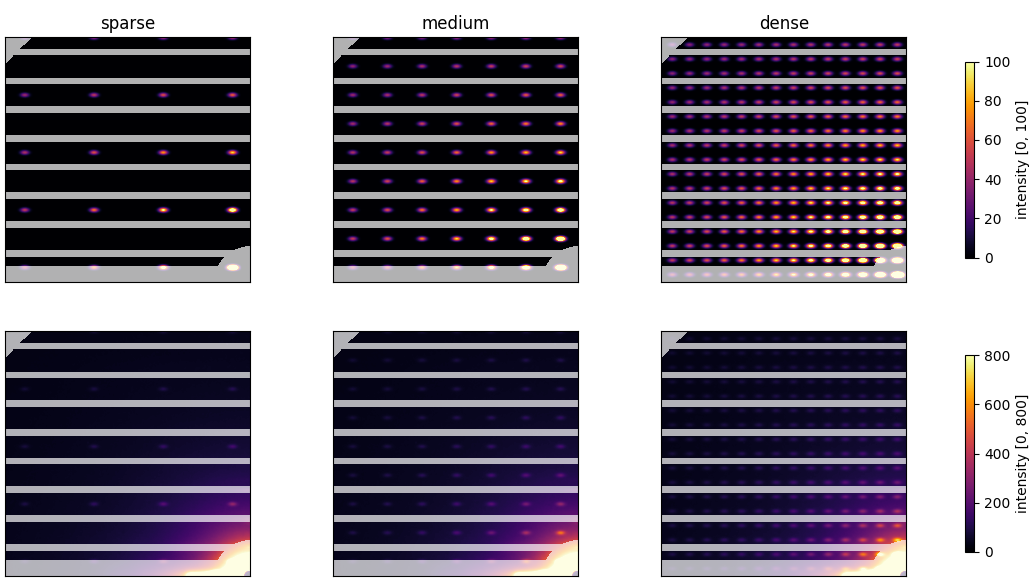
\includegraphics[width=0.8\columnwidth]{figs/Fig1_synthetic_data_variations_v2.png}
\caption{Representative placement of synthetic features, visible as small bright elliptical dots. The figure also shows masking of the central beam region, equatorial streak background, and layer line regions (see Section~\ref{sec:masking}). The synthetic features are distributed to sample background-dominated regions while avoiding overlap with real diffraction signal. Top: synthetic features. Bottom: real diffraction image with superimposed synthetic features. The three columns represent different synthetic feature placement frequencies: sparse, medium, and dense. The intensity of the synthetic features is increased for better visibility.}
\label{fig:synthetic_structures}
\end{figure}

\label{sec:masking}
\begin{table}[h]
\caption{Sensitivity of the aggregate loss to variations in synthetic signal parameters evaluated on a subset of the data.
Average loss values are reported for ten images from three datasets.
For each parameter variation, all other parameters were held at their medium setting.
Results show that the default settings produce consistently low loss values and stable method rankings. `LL' stands for layer lines.}
\label{tab:variations}
\centering
\footnotesize
% \tiny
\setlength{\tabcolsep}{4pt}
\renewcommand{\arraystretch}{1.0}
% \begin{tabularx}{\linewidth}{@{}>{\RaggedRight}Xl>{\RaggedRight}Xc@{}}
\begin{tabular}{@{}llll@{}}
\toprule
\textbf{Parameter} & \textbf{Variation} & \textbf{Setting} & \textbf{Loss} \\ \midrule
Horizontal extent $\sigma_x$ & Short & $I_{1,0}/7$ & $0.51 \pm 0.16$ \\
& Medium & $I_{1,0}/5$ & $0.51 \pm 0.12$ \\
& Long & $I_{1,0}/3$ & $0.53 \pm 0.16$ \\ \midrule
Vertical extent $\sigma_y$ & Thin & $\mathrm{M1}/20$ & $0.50 \pm 0.13$ \\
& Medium & $\mathrm{M1}/10$ & $0.51 \pm 0.12$ \\
& Thick & $\mathrm{M1}/5$ & $0.51 \pm 0.13$  \\ \midrule
Sampling frequency & Sparse & Every two LL. & $0.51 \pm 0.12$ \\
$(f_x, f_y)$ & Medium & Every LL. & $0.51 \pm 0.12$ \\
& Dense & Two between LL. & $0.52 \pm 0.13$ \\
\bottomrule
% \end{tabularx}
\end{tabular}
\end{table}

\subsubsection{Region-Specific Masking}
Accurate calculation of evaluation metrics requires separating regions containing diffraction signal from those dominated by background or artifacts. To achieve this, multiple complementary masks are applied. \textit{Main signal mask} is an annulus excluding the beam center and detector edges ($r_{\mathrm{min}}$, $r_{\mathrm{max}}$). This mask excludes regions containing non-representative or saturated signal. \textit{Equator mask} is a rectangle aligned with the equator. The equatorial streak is treated separately, since it is typically more intense than the surrounding diffuse background. \textit{Synthetic mask} consists rectangles of extent $2\sigma$ around each injected feature. \textit{Real-feature mask} consists of bands at layer-line positions with widths set from estimated FWHM via perpendicular projections. This mask is used to avoid contamination from real diffraction signal. Together, these masks restrict metric evaluation to regions dominated by background, ensuring that evaluation reflects background subtraction quality rather than signal content.

\subsection{Optimization Procedure}
\label{sec:optimization_procedure}

This subsection describes how the evaluation metrics are combined into a single objective function, which is minimized to tune each method's parameters. An overview of the evaluation and optimization workflow used to identify optimal background subtraction parameters for muscle fiber diffraction patterns is shown in Figure~\ref{fig:flow}.

\subsubsection{Aggregate Loss Function}

Background subtraction quality is quantified using a weighted aggregate loss function that combines the normalized metrics defined in the evaluation framework. The objective function is constructed to balance physically meaningful constraints, artifact suppression, and preservation of faint diffraction signal. It is defined as
\begin{equation}
%\begin{aligned}
L =\;
\lambda_1\, S_{\mathrm{BG}}
+ \lambda_2\, f_{\mathrm{neg,con}}
+ \lambda_3\, f_{\mathrm{neg,syn}}
+ \lambda_4\, \mathrm{NMSE}_{\mathrm{syn}}
+ \lambda_5\, \bigl(1 - f_{B}\bigr),
%\end{aligned}
\end{equation}
where each metric is normalized by its average value across datasets prior to aggregation, ensuring comparable scale during optimization. The normalization averages are obtained using a calibration subset of images from each dataset. The weights $\lambda_i$ encode the relative importance of different physical and algorithmic considerations and may be adjusted to reflect user priorities. We started off with equal weights and adjusted them based on visual inspection of the results. Although the optimization is driven by quantitative metrics, visual inspection remains necessary to identify artifacts that are difficult to capture numerically, such as faint negative excursions or distortion of layer lines or to adjust dataset specific weights. The final weights used in this study are nearly identical across datasets, with only the $\lambda_4$ term (NMSE$_{\mathrm{syn}}$) varying to a small degree. The most common combination is $[\lambda_1, \lambda_2, \lambda_3, \lambda_4, \lambda_5] = [0.1, 0.05, 0.05, 0.01, 0.8]$. Visualization of the results based on the optimization of individual metrics, shown in Appendix Figure~\ref{fig:example_1img_metrics}, reflects that no single metric is sufficient to guide optimization.

\subsubsection{Parameter Optimization}

The aggregate loss function is minimized to identify optimal parameter values for each background subtraction method. Because these methods typically involve non-differentiable operations and discrete parameter choices (e.g.\ window size or number of smoothing cycles), gradient-based optimization is not well suited. Instead, direct search strategies that rely solely on function evaluations are employed, despite their higher computational cost. To minimize $L$ we use a coordinate-descent strategy in which parameters are optimized sequentially, in the order of their estimated significance, with all other parameters held fixed at their current best values. Input parameters are either integer-valued or exhibit no qualitative sensitivity to fractional changes. For each algorithm, predefined initial values and parameter bounds are specified. Across the datasets considered here, optimized parameter values for all methods fall within the range $[0, 2000]$, although these bounds may be adjusted for alternative implementations. Optimization proceeds using a decreasing multi-resolution step-size schedule, with step sizes ranging from 150 to 1. As the loss value improves, the step size is restarted from fine to coarse to avoid getting stuck in local minima. Images are processed in parallel using multiprocessing to reduce overall runtime. Additionally, for further computational efficiency, images are downsampled prior to background estimation and evaluated at full resolution. Only the estimated background is downsampled; it is then subtracted from the original-resolution image to preserve diffraction signal fidelity. The impact of downsampling depends on the background subtraction method. Downsampling is applied only when it leads to reduced loss values: a factor of 2 is used for the background subtraction methods: G-ILPF, B-ILPF, RW, and WTH; and no downsampling for CS, RCH, or AVG.



\subsection{Experimental Design}
\label{sec:experimental_design}

\begin{wrapfigure}{r}{0.5\linewidth}
\centering
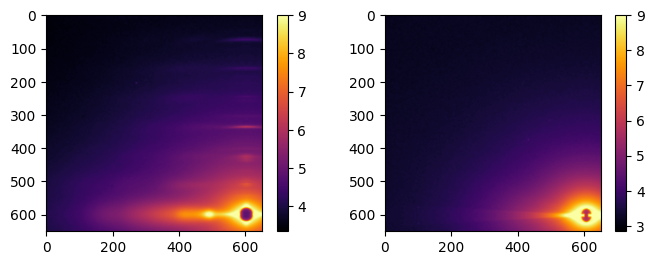
\includegraphics[width=\linewidth]{figs/Fig3_image_filtering_quarter2.png}
\caption{Examples of included and excluded diffraction images based on manual assessment of the presence of well-defined diffraction features. Images on the left contain clear equatorial and layer line features suitable for quantitative analysis, whereas images on the right lack discernible diffraction structure and are therefore excluded from evaluation.}
\label{fig:img_filter}
\end{wrapfigure}

We optimize a representative set of background subtraction algorithms commonly used for fiber diffraction analysis, implemented in MuscleX Quadrant Folding~\citep{JiratrakanvongEtAl2024}, which is based on algorithms originally developed within the CCP13 software suite~\citep{rajkumar2007fibrefix}. The selected methods span a range of underlying assumptions and algorithmic strategies, providing a broad basis for comparison. A summary of the tested algorithms is provided in Table~\ref{tab:algorithms}. Any newly developed or improved method for background subtraction in fiber diffraction can be evaluated using the proposed framework, providing a consistent basis.

To assess robustness across experimental conditions, we selected a diverse set of muscle fiber diffraction datasets acquired using different detectors and sample environments, including samples measured in solution, buffer, and air. The data used in our study were taken on either the Mar 165 CCD detector (Rayonix Inc.) or the EIGER X 9M pixel array detector (Dectris AG). Images were manually filtered to exclude frames lacking clearly defined diffraction features, as preservation of diffraction peaks is required for meaningful evaluation of background subtraction performance. Table~\ref{tab:datasets} lists datasets used in this study. Frames lacking clearly defined diffraction features were excluded, as shown in Figure~\ref{fig:img_filter}. For optimization and evaluation, close to 50 images were selected from each dataset.

Applying guided filtering to smooth diffraction images prior to background estimation improves performance for several non-parametric methods, particularly the white top-hat (WTH) filter, which is sensitive to high-frequency noise. In this study, a smoothing filter was applied to all studied background subtraction methods as it produced visually plausible results. Downsampling the patterns has a similar effect, reducing computational load while smoothing the pattern and thus improving performance. Importantly, smoothing is applied only to estimate the background; the background-subtracted image is computed using the original, unsmoothed data, ensuring that diffraction features are preserved.

\begin{table}[h]
\caption{Experimental datasets used in the analysis. Images lacking clearly defined diffraction features were excluded. A subset was used for experiments.}
\label{tab:datasets}
\centering
\footnotesize
\setlength{\tabcolsep}{4pt}
\renewcommand{\arraystretch}{1.0}
\begin{tabular}{@{}llccccc@{}}
\toprule
\textbf{Name} & \textbf{Muscle Type} & \textbf{Detector} & \textbf{Environment} & \textbf{Total} & \textbf{Filtered} & \textbf{Subselected} \\ \midrule
2025\_0227 & Skinned Pig Cardiac & Mar 165 & Solution & 685 & 345 & 50 \\
P2\_F6\_639 & Intact Pig Cardiac & EIGER X 9M & Solution & 120 & 120 & 50 \\
P3\_F4\_675 & Intact Pig Cardiac & EIGER X 9M & Solution & 120 & 120 & 48 \\
2024\_0508 & Skinned Pig Cardiac & Mar 165 & Solution & 267 & 246 & 50 \\
2024\_1213 & Skinned Pig Cardiac & Mar 165 & Buffer & 242 & 188 & 45 \\
2024\_1213 & Skinned Pig Cardiac & Mar 165 & Air & 287 & 237 & 50 \\
2025\_0402 & Skinned Pig Cardiac & Mar 165 & Solution & 640 & 640 & 50 \\
2026\_0409 & Skinned Mouse Cardiac & Mar 165 & Air & 304 & 304 & 50 \\
2026\_0409 & Skinned Mouse Cardiac & Mar 165 & Solution & 325 & 325 & 50 \\
2022\_1028 & Intact Mouse Skeletal & Mar 165 & Solution & 1282 & 1282 & 50 \\
MPLL & Skinned Pig Cardiac & Mar 165 & Solution & 63 & 63 & 50 \\ \midrule
\textbf{Total} & -- & -- & -- & \textbf{3111} & \textbf{2108} & \textbf{534} \\
\bottomrule
\end{tabular}
\end{table}


% \subsection{Equatorial Streak}
% \label{sec:equatorial_streak}


\subsection{Iterative Two-Stage Background Subtraction}
\label{sec:two_stage}

This subsection describes an approach for removing background across the whole pattern by jointly modeling the anisotropic equatorial streak and the surrounding isotropic general background. Fitting each component once and treating the residual as final is not sufficient: the equator and the general background are not spatially independent, so a single equatorial fit is biased by the presence of the general background beneath it, and a general-background fit performed only once after equator subtraction still leaves a substantial fraction of isotropic scattering uncorrected in and around the equatorial region. To address this, the equatorial and general-background fits are refined iteratively, each using the other's current estimate as input, until both have converged to a consistent decomposition of the whole pattern into the individual background components.

\subsubsection{Parametric Background Modelling}

Each iteration round requires an initial estimate of the general background to isolate the equatorial streak for fitting. Scattering from isotropic components in diffraction experiments is expected to produce approximately circular intensity distributions, which are naturally described in polar coordinates. In muscle fiber diffraction data, the general background is observed to be nearly circularly symmetric, with mild elongation along the equatorial direction. The parametric model that produced flexible yet plausible results for a variety of datasets combines a power-law decay with a low-order orthogonal polynomial expansion,
\begin{equation}
B(q) = \sum_{j=0}^{3} a_j\, T_j(\tilde q) + A_{\mathrm{p}}\, (q + q_0)^{-p},
\end{equation}
where $T_j$ denotes Chebyshev polynomials and $q$ is the radial coordinate. Model parameters are estimated by least-squares fitting to radial intensity projections. To account for slight equatorial elongation, projections are integrated between angles $0-5^{\circ}$ from the meridian, $5-10^{\circ}$, and $10-60^{\circ}$. Two-dimensional background is interpolated using the one-dimensional fitted projections and subtracted from the original image, resulting in a background-subtracted image that retains the equatorial streak while removing the general background. This step is crucial to ensure that the subsequent parametric modeling of the equatorial streak is not confounded by the presence of the general background, which could bias parameter estimation and lead to suboptimal subtraction results. This one-dimensional projection-based estimate, $B_0$, is used only to seed the first round of the iterative refinement described next; from the second round onward it is replaced by the two-dimensional general-background fit.

\subsubsection{Equatorial Streak Modeling}

Parametric modeling of equatorial streaks has previously been developed for polymer diffraction data using elliptical coordinates and Pearson VII functions~\citep{MurthyZeroGrubb1997}. Rod-like particles in both polymer and biological samples produce streak-like diffraction features in reciprocal space, suggesting that similar models may be applicable to muscle fiber diffraction. The streak is modeled using the parametric form used for polymer diffraction data in elliptical coordinates~\citep{MurthyZeroGrubb1997} and fitted via least-squares minimization. Because two-dimensional fitting is computationally intensive, the diffraction patterns are downsampled by a factor of two during the fitting stage. Rather than finalizing the fit after a single pass, the equatorial streak and the general background are then refined together, as described next.

\begin{figure}[h]
\centering
\resizebox{0.5\linewidth}{!}{%
\begin{tikzpicture}[
  font=\scriptsize,
  every node/.style={align=center},
  box/.style={draw, rounded corners=2pt, minimum height=6mm, minimum width=14mm, fill=gray!6, inner sep=2pt},
  lbl/.style={font=\bfseries\footnotesize, align=right, text width=15mm},
  arr/.style={-{Stealth[length=1.6mm]}, thick}
]

\node[lbl] at (-1.9,0) {Round 1\\(seed $B_0$)};
\node[box] (img) at (0,0)   {image};
\node[box] (b0)  at (1.7,0) {$B_0$};
\node[box] (e1)  at (3.4,0) {$E_1$};
\node[box] (g1)  at (5.1,0) {$G_1$};

\node[lbl] at (-1.9,-1.6) {Rounds\\$2,\dots,N$};
\node[box] (e2)   at (1.7,-1.6) {$E_k$};
\node[box] (g2)   at (3.4,-1.6) {$G_k$};
\node[box] (dots) at (5.1,-1.6) {repeat};

\node[lbl] at (-1.9,-3.2) {Select};
\node[box] (sel) at (3.4,-3.2) {best round};

\node[box] (fin)  at (2.55,-4.5) {final};
\node[box] (safe) at (4.25,-4.5) {safe};

\draw[arr] (img) -- (b0);
\draw[arr] (b0)  -- (e1);
\draw[arr] (e1)  -- (g1);
\draw[arr] (g1.south) -- ++(0,-0.4) -| (e2.north);
\draw[arr] (e2) -- (g2);
\draw[arr] (g2) -- (dots);
\draw[arr] (dots.south) -- ++(0,-0.4) -| (sel.north);
\draw[arr] (sel.south) -- (fin.north);
\draw[arr] (sel.south) -- (safe.north);

\end{tikzpicture}%
}
\caption{Iterative two-stage background subtraction pipeline. Round 1 is seeded by the projection-based general background $B_0$ (Parametric Background Modelling), giving the first equatorial fit $E_1$ and general-background fit $G_1$. In rounds $2,\dots,N$, $E_k$ is fitted on $\mathrm{img}-G_{k-1}$ and $G_k$ on $\mathrm{img}-E_k$. The best round is selected using an oversubtraction-based criterion, giving the final residual $\mathrm{img}-E-G$ (``final'') and a variant with the background scaled to further reduce oversubtraction if present(``safe'').}
\label{fig:two_stage_pipeline}
\end{figure}

\subsubsection{Iterative Refinement}

Figure~\ref{fig:two_stage_pipeline} summarizes the resulting pipeline. After the first round, seeded by the projection-based general background $B_0$ above, each subsequent round $k$ re-fits the equatorial streak $E_k$ on $\mathrm{img} - G_{k-1}$ and the general background $G_k$ on $\mathrm{img} - E_k$, using the two-dimensional general-background fit from the previous round in place of the projection-based seed. From the second round onward, the general background is parameterized directly in two dimensions as an exponential decay plus a flat baseline plus one additional radially symmetric term, selected per image from a small set of candidate forms (Lorentzian, power-law, and stretched-exponential). The candidate that minimizes oversubtraction, with fit quality used only as a tie-break, is selected independently for each image, since no single form was found to be best across all datasets in a model-comparison screen of the candidate set.

This adaptive, per-image selection is appropriate when the goal is the best possible background fit for each individual image. If instead the goal is to compare the fitted background parameters themselves across images or datasets -- for example, to study how the general-background shape changes with experimental condition -- the functional form should be fixed to a single common choice across all images, since the fitted parameters are only directly comparable when they describe the same functional form. The best-performing round is selected automatically using an oversubtraction-based criterion, and two independent post-fit scale factors -- applied to the equatorial streak and to the general baseline -- guard against residual oversubtraction without requiring a refit. An example of the resulting fitted backhgrounds is shown in Figure~\ref{fig:visual_eq_none}.


\begin{figure}[h]
\centering
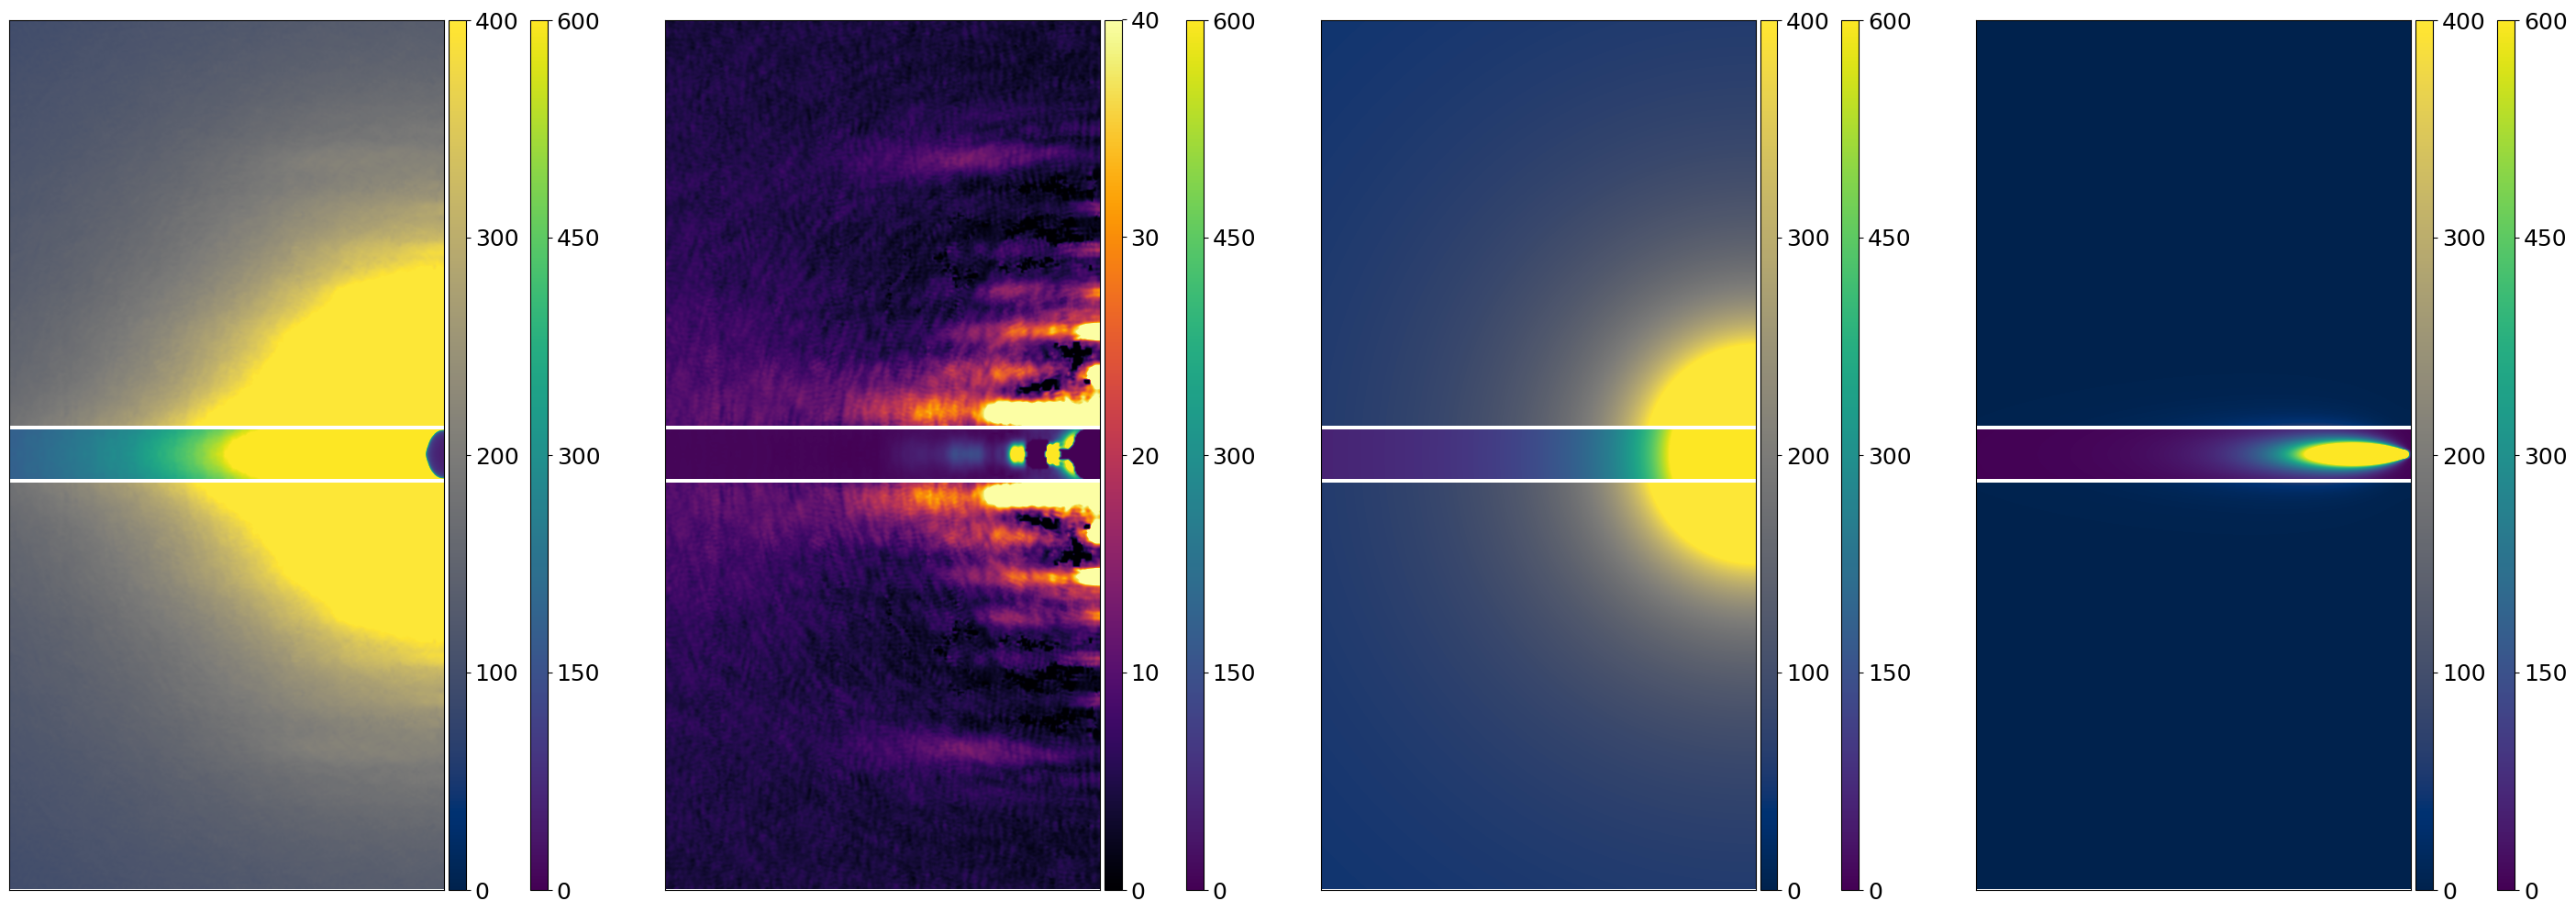
\includegraphics[width=0.7\linewidth]{figs/Fig6_visual_eq_Weikang_4_half_v3.png}
\hspace{0.01\linewidth}
\caption{Examples of background subtraction outcomes with parametric fitted background. Left to right: original image before subtraction, background-sutracted pattern, fitted general background, and fitted equatorial streak. Two scales are used for visualization due to high intensity differences between the equatorial streak and the rest of the pattern. Most of the background is subtracted with some high-angle residual background left over. }
\label{fig:visual_eq_none}
\end{figure}


%%%%%%%%%%%%%%%%%%%%%%%%%%%%%%%%%%%%%%%%%%
\section{Conclusions}
\label{sec:conclusion}

We presented a quantitative, physics-informed framework for the evaluation and optimization of background subtraction methods in muscle fiber diffraction images, replacing subjective visual assessment with reproducible metrics, synthetic-signal validation, and an automated parameter search. Out of the tested non-parametric background subtraction methods, no single method dominated universally, which is the central argument for a framework that selects and tunes methods per dataset rather than prescribing fixed algorithm and parameters.

Combining the iterative two-stage equatorial-general fit with a non-parametric framework method extends background subtraction across the whole pattern, including the equatorial streak, and improved on the RCH baseline in both the general-background region and the equatorial region itself, since the parametric and non-parametric approaches address different failure modes and are most effective combined rather than used in isolation.

Overall, the proposed framework establishes an objective and reproducible foundation for background subtraction in muscle fiber diffraction. Although the background removal is not fully automated, it is supported by a quantitative metric for evaluating subtraction quality. The new approach makes any required manual adjustment more intuitive, since the parameters have clear physical meaning. In addition, the system automatically searches over candidate algorithms and parameter values, reducing the extent of manual intervention needed.

The framework has been integrated into the MuscleX version 2.0.0~\citep{lee2019musclex}, where it runs background subtraction with quantitative evaluation and parameter optimization as part of routine analysis while leaving users free to review results and make adjustments. While  this implementation is specific to muscle diffraction, the underlying metrics and optimization procedure are based on general signal and background properties, and the same approach could be extended to other fiber diffraction and imaging contexts where a structured, non-uniform background must be separated from weak signal without access to ground truth.

%%%%%%%%%%%%%%%%%%%%%%%%%%%%%%%%%%%%%%%%%%
% \section{Patents}

%%%%%%%%%%%%%%%%%%%%%%%%%%%%%%%%%%%%%%%%%%
\vspace{6pt} 

%%%%%%%%%%%%%%%%%%%%%%%%%%%%%%%%%%%%%%%%%%
%% optional
\supplementary{Code for the optimization framework and the evaluation metrics is available at \url{https://github.com/biocatiit/musclex}.}
% The following supporting information can be downloaded at \linksupplementary{s1}. 

% Only for journal Methods and Protocols:
% If you wish to submit a video article, please do so with any other supplementary material.
% \supplementary{The following supporting information can be downloaded at \linksupplementary{s1}, Figure S1: title; Table S1: title; Video S1: title. A supporting video article is available at doi: link.}

% Only used for preprtints:
% \supplementary{The following supporting information can be downloaded at the website of this paper posted on \href{https://www.preprints.org/}{Preprints.org}.}

% Only for journal Hardware:
% If you wish to submit a video article, please do so with any other supplementary material.
% \supplementary{The following supporting information can be downloaded at \linksupplementary{s1}, Figure S1: title; Table S1: title; Video S1: title.\vspace{6pt}\\
%\begin{tabularx}{\textwidth}{lll}
%\toprule
%\textbf{Name} & \textbf{Type} & \textbf{Description} \\
%\midrule
%S1 & Python script (.py) & Script of python source code used in XX \\
%S2 & Text (.txt) & Script of modelling code used to make Figure X \\
%S3 & Text (.txt) & Raw data from experiment X \\
%S4 & Video (.mp4) & Video demonstrating the hardware in use \\
%... & ... & ... \\
%\bottomrule
%\end{tabularx}
%}

%%%%%%%%%%%%%%%%%%%%%%%%%%%%%%%%%%%%%%%%%%
\authorcontributions{Conceptualization and methodology, G.A, T.C.I. and I.K.;.; software, I.K. and G.A.; validation, T.C.I.; formal analysis, G.A, T.C.I. and I.K.; resources, T.C.I.; data curation, T.C.I.; writing---original draft preparation, I.K.; writing---review and editing, G.A and T.C.I.; visualization, I.K. and T.C.I.; supervision, G.A and T.C.I.; funding acquisition, T.C.I. All authors have read and agreed to the published version of the manuscript.}

\funding{This research was funded by the US National Institutes of Health grant number R01GM144555 (TI).}

\institutionalreview{Not applicable.}

\informedconsent{Not applicable.}

\dataavailability{The data presented in this study are available on request from the corresponding author. The source code for the optimization framework and the evaluation metrics is available at \url{https://github.com/biocatiit/musclex}.} 
% A part of the original data presented in the study are openly available in [repository name] at [link], reference number [reference number]. The remaining data presented in this study are available on request from the corresponding author. 

%\durcstatement{Current research is limited to the [please insert a specific academic field, e.g., XXX], which is beneficial [share benefits and/or primary use] and does not pose a threat to public health or national security. Authors acknowledge the dual-use potential of the research involving xxx and confirm that all necessary precautions have been taken to prevent potential misuse. As an ethical responsibility, authors strictly adhere to relevant national and international laws about DURC. Authors advocate for responsible deployment, ethical considerations, regulatory compliance, and transparent reporting to mitigate misuse risks and foster beneficial outcomes.}

% Only for journal Nursing Reports
%\publicinvolvement{Please describe how the public (patients, consumers, carers) were involved in the research. Consider reporting against the GRIPP2 (Guidance for Reporting Involvement of Patients and the Public) checklist. If the public were not involved in any aspect of the research add: ``No public involvement in any aspect of this research''.}
%
%% Only for journal Nursing Reports
%\guidelinesstandards{Please add a statement indicating which reporting guideline was used when drafting the report. For example, ``This manuscript was drafted against the XXX (the full name of reporting guidelines and citation) for XXX (type of research) research''. A complete list of reporting guidelines can be accessed via the equator network: \url{https://www.equator-network.org/}.}
%
%% Only for journal Nursing Reports
%\useofartificialintelligence{Please describe in detail any and all uses of artificial intelligence (AI) or AI-assisted tools used in the preparation of the manuscript. This may include, but is not limited to, language translation, language editing and grammar, or generating text. Alternatively, please state that “AI or AI-assisted tools were not used in drafting any aspect of this manuscript”.}

\acknowledgments{During the preparation of this manuscript and the accompanying analysis code, the author(s) used Claude (Anthropic) for language editing of the text and for coding assistance, including code completions and the writing of utility functions. The authors have reviewed and edited the output and take full responsibility for the content of this publication.}

\conflictsofinterest{The authors declare no conflicts of interest. The funders had no role in the design of the study; in the collection, analyses, or interpretation of data; in the writing of the manuscript; or in the decision to publish the~results.} 

%%%%%%%%%%%%%%%%%%%%%%%%%%%%%%%%%%%%%%%%%%
%% Optional

%% Only for journal Encyclopedia
%\entrylink{The Link to this entry published on the encyclopedia platform.}

\abbreviations{Abbreviations}{%
The following abbreviations are used in this manuscript:\\
\noindent 
\begin{tabular}{@{}ll}
\footnotesize
AVG & Mean value of non-masked pixels (baseline)\\
B-ILPF & Boxcar iterative low-pass filter\\
CCD & Charge-coupled device\\
CS & Circularly symmetric\\
CV & Coefficient of variation\\
FWHM & Full width at half maximum\\
G-ILPF & Gaussian iterative low-pass filter\\
LL & Layer line\\
NMSE & Normalized mean squared error\\
RCH & Radial convex hull\\
RW & Roving window\\
WTH & White top-hat filter
\end{tabular}
}

%%%%%%%%%%%%%%%%%%%%%%%%%%%%%%%%%%%%%%%%%%
%% Optional
\appendixtitles{no} % Leave argument "no" if all appendix headings stay EMPTY (then no dot is printed after "Appendix A"). If the appendix sections contain a heading then change the argument to "yes".
\appendixstart
\appendix
\section[\appendixname~\thesection]{}
% \subsection[\appendixname~\thesubsection]{}

Sensitivity to the synthetic signal parameters was also evaluated. Table~\ref{tab:synthetic_variations} summarizes results obtained under different synthetic feature configurations. The relatively small changes in aggregate loss across these conditions indicate that the evaluation framework is not overly sensitive to the precise choice of synthetic signal parameters.

\begin{table}[h]
\centering
\footnotesize
\begin{tabular}{lcccccccr}
\hline
\textbf{Samp. Freq.} & \textbf{($\sigma_x$, $\sigma_y$)} & \textbf{Loss} & $\mathbf{NMSE}_{\mathbf{syn}}$ & $\mathbf{f}_{\mathbf{neg,con}}$ & $\mathbf{f}_{\mathbf{neg,syn}}$ & $\mathbf{1-f_B}$ & $\mathbf{S}_{\mathbf{BG}}$ \\
\hline
dense & (5, 10) & $0.52 \pm 0.13$ & $5.10 \pm 4.57$ & $0.90 \pm 0.65$ & $1.09 \pm 0.39$ & $0.24 \pm 0.12$ & $1.89 \pm 0.33$ \\
medium & (5, 5) & $0.51 \pm 0.13$ & $4.17 \pm 4.21$ & $0.89 \pm 0.66$ & $1.07 \pm 0.41$ & $0.26 \pm 0.14$ & $1.82 \pm 0.26$ \\
medium & (3, 10) & $0.53 \pm 0.16$ & $5.36 \pm 5.22$ & $0.90 \pm 0.67$ & $1.09 \pm 0.35$ & $0.27 \pm 0.17$ & $1.84 \pm 0.19$ \\
medium & (7, 10) & $0.51 \pm 0.16$ & $3.70 \pm 4.47$ & $0.91 \pm 0.67$ & $1.01 \pm 0.40$ & $0.26 \pm 0.17$ & $1.87 \pm 0.20$ \\
medium & (5, 10) & $0.51 \pm 0.12$ & $3.61 \pm 3.52$ & $0.91 \pm 0.67$ & $1.05 \pm 0.40$ & $0.25 \pm 0.15$ & $1.85 \pm 0.20$ \\
medium & (5, 20) & $0.50 \pm 0.13$ & $3.33 \pm 3.41$ & $0.91 \pm 0.67$ & $1.05 \pm 0.40$ & $0.25 \pm 0.15$ & $1.86 \pm 0.20$ \\
sparse & (5, 10) & $0.51 \pm 0.12$ & $3.61 \pm 3.52$ & $0.91 \pm 0.67$ & $1.05 \pm 0.40$ & $0.25 \pm 0.15$ & $1.85 \pm 0.20$ \\
\hline
\end{tabular}
\caption{Sensitivity of the evaluation framework to variations in synthetic signal parameters. Values are reported as mean $\pm$ standard deviation across datasets. The purpose of this table is to demonstrate robustness of the aggregate loss to reasonable changes in synthetic feature configuration.}
\label{tab:synthetic_variations}
\end{table}

% \section[\appendixname~\thesection]{}
Figure \ref{fig:example_1img_metrics} shows an example of background subtraction outcomes for a single image from dataset 2025\_0227 when guided using metrics individually or a combination of the two most significant. No single metric dominates performance across all methods, underscoring the need for a composite evaluation criterion.

% \section[\appendixname~\thesection]{}
Figure \ref{fig:example_1img_all_bg} shows an example of background subtraction outcomes for different methods on a single image from dataset 2025\_0227. 

\begin{figure}[H]
\centering
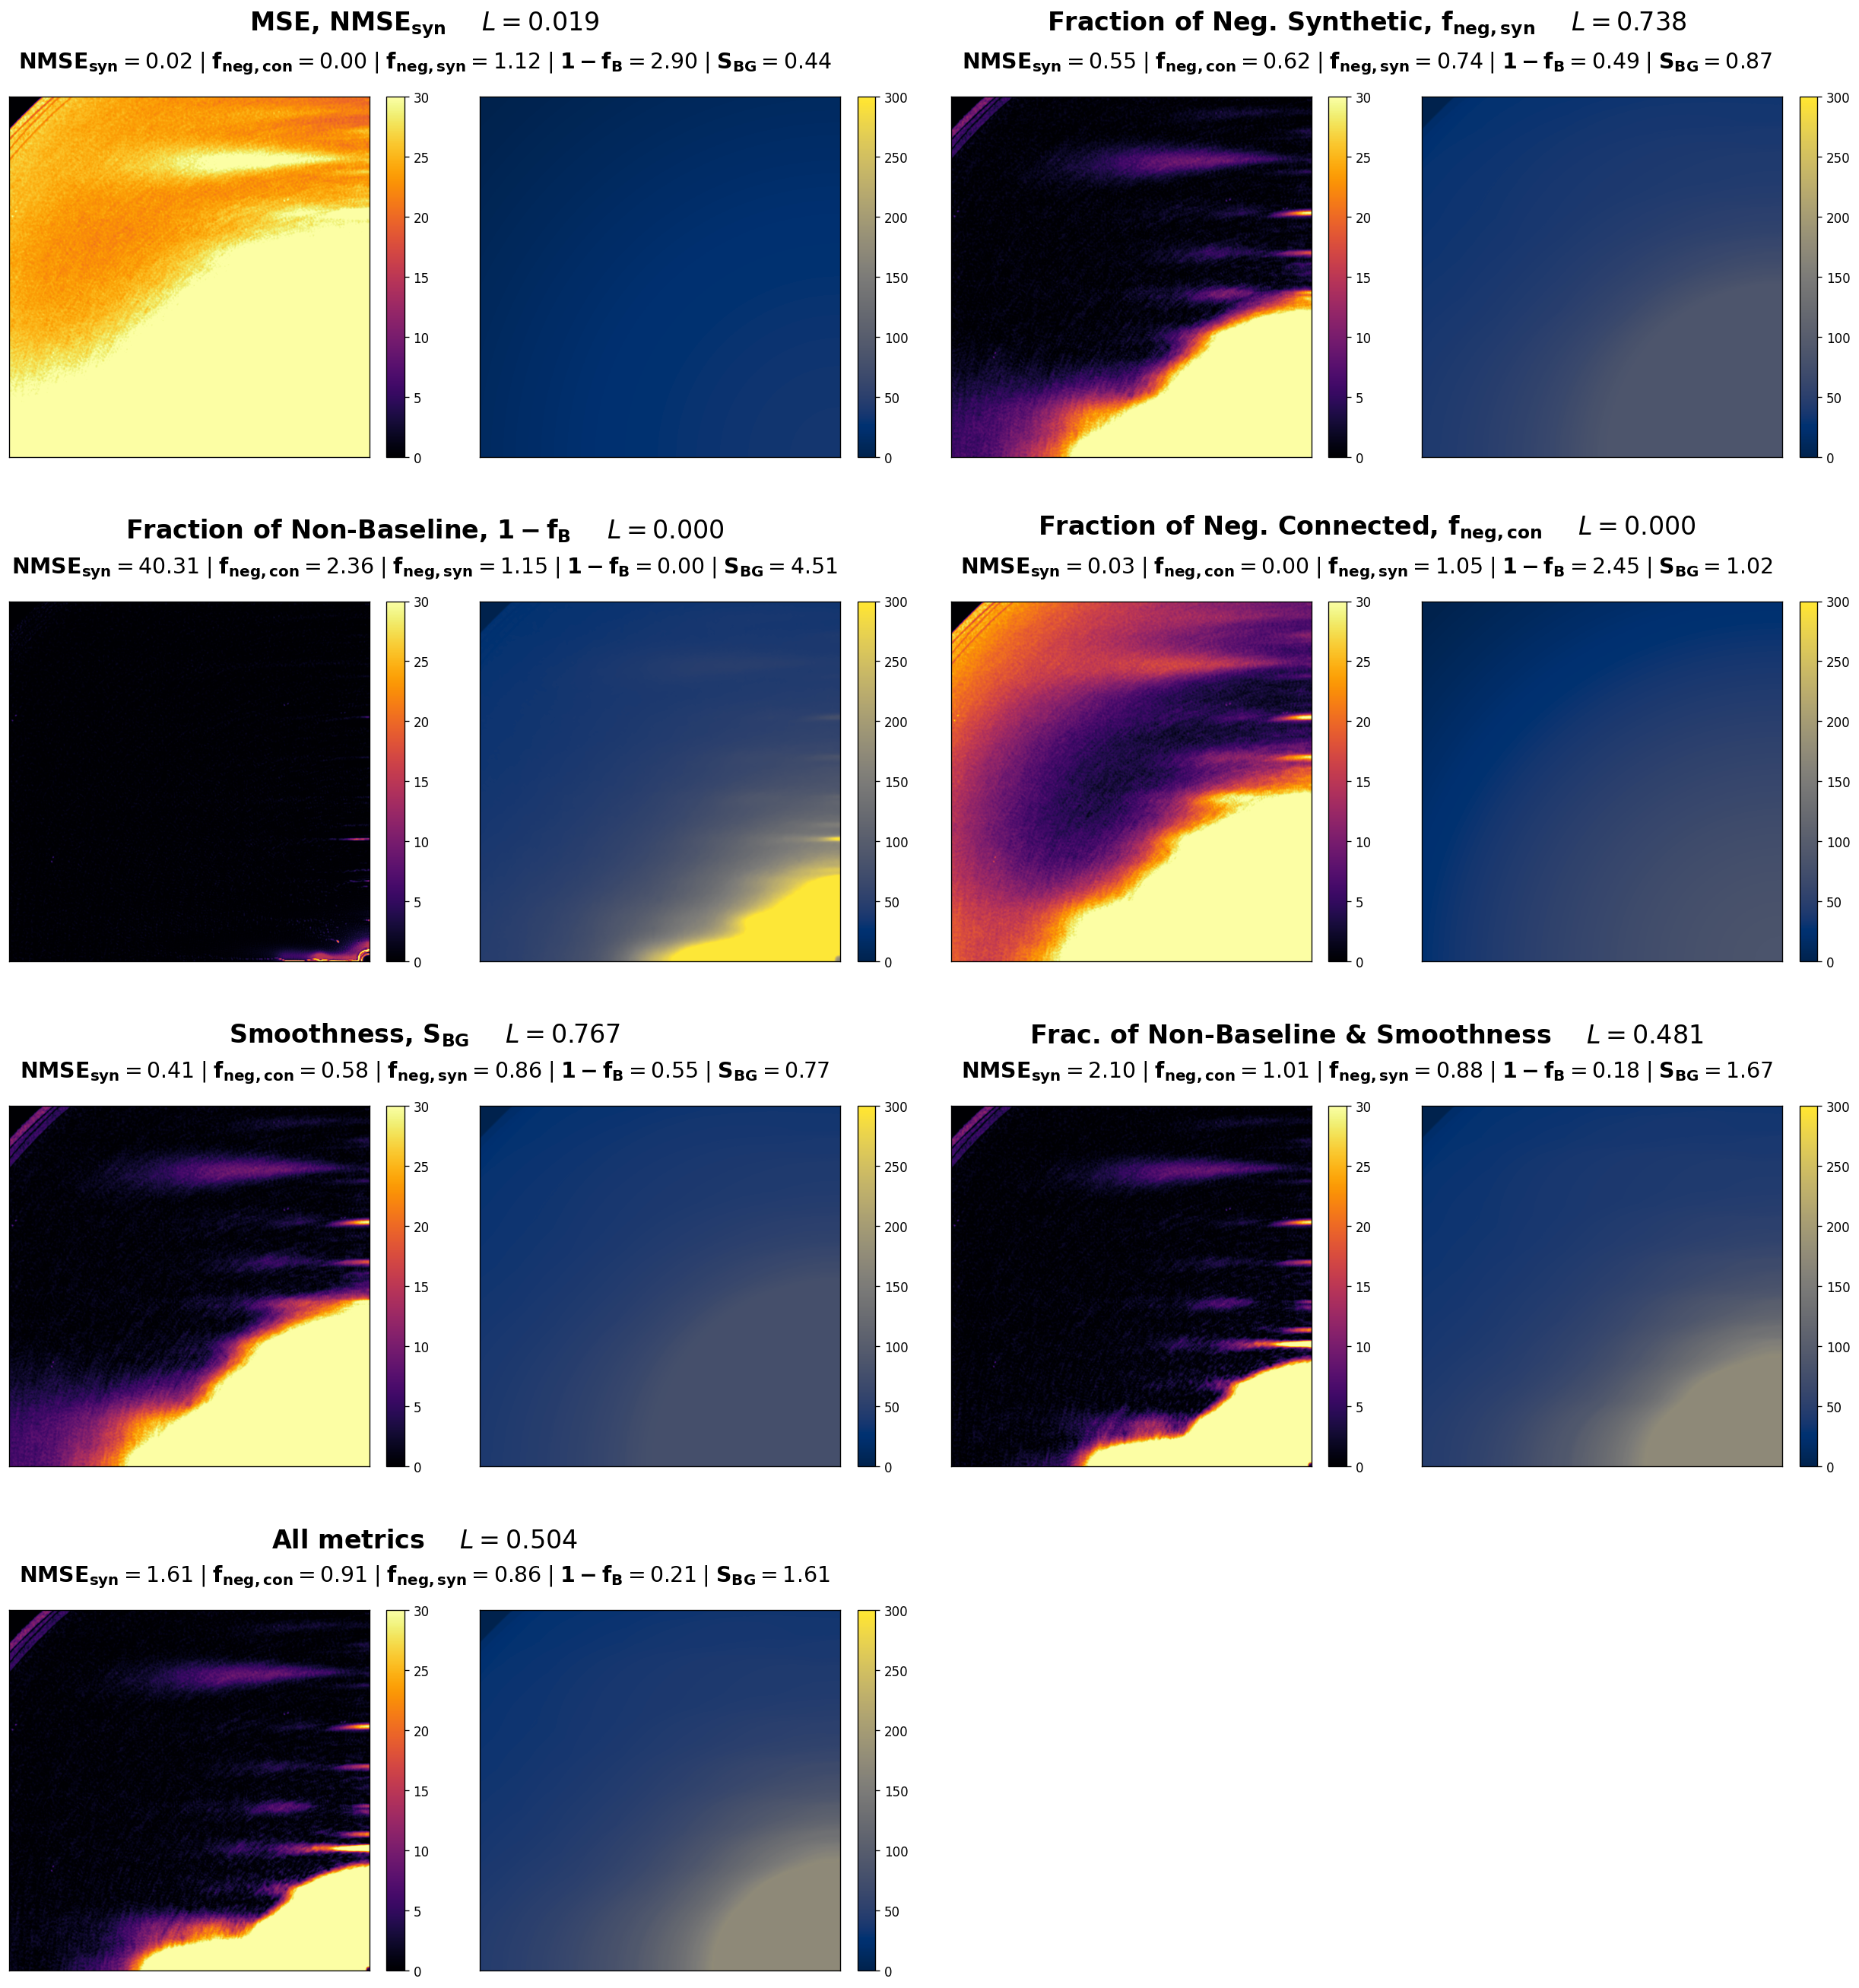
\includegraphics[width=0.74\textwidth]{figs/Fig12_appendix_individual_metrics_v3.png}
\caption{\footnotesize  Image sample from dataset 2025\_0227 when guided using metrics individually or a combination of the two most significant. Left of each pair: Background removed image. Right: Background.}
\label{fig:example_1img_metrics}
\end{figure}

\begin{figure}[H]
\centering
\begin{minipage}{0.48\textwidth}
    \raggedleft
    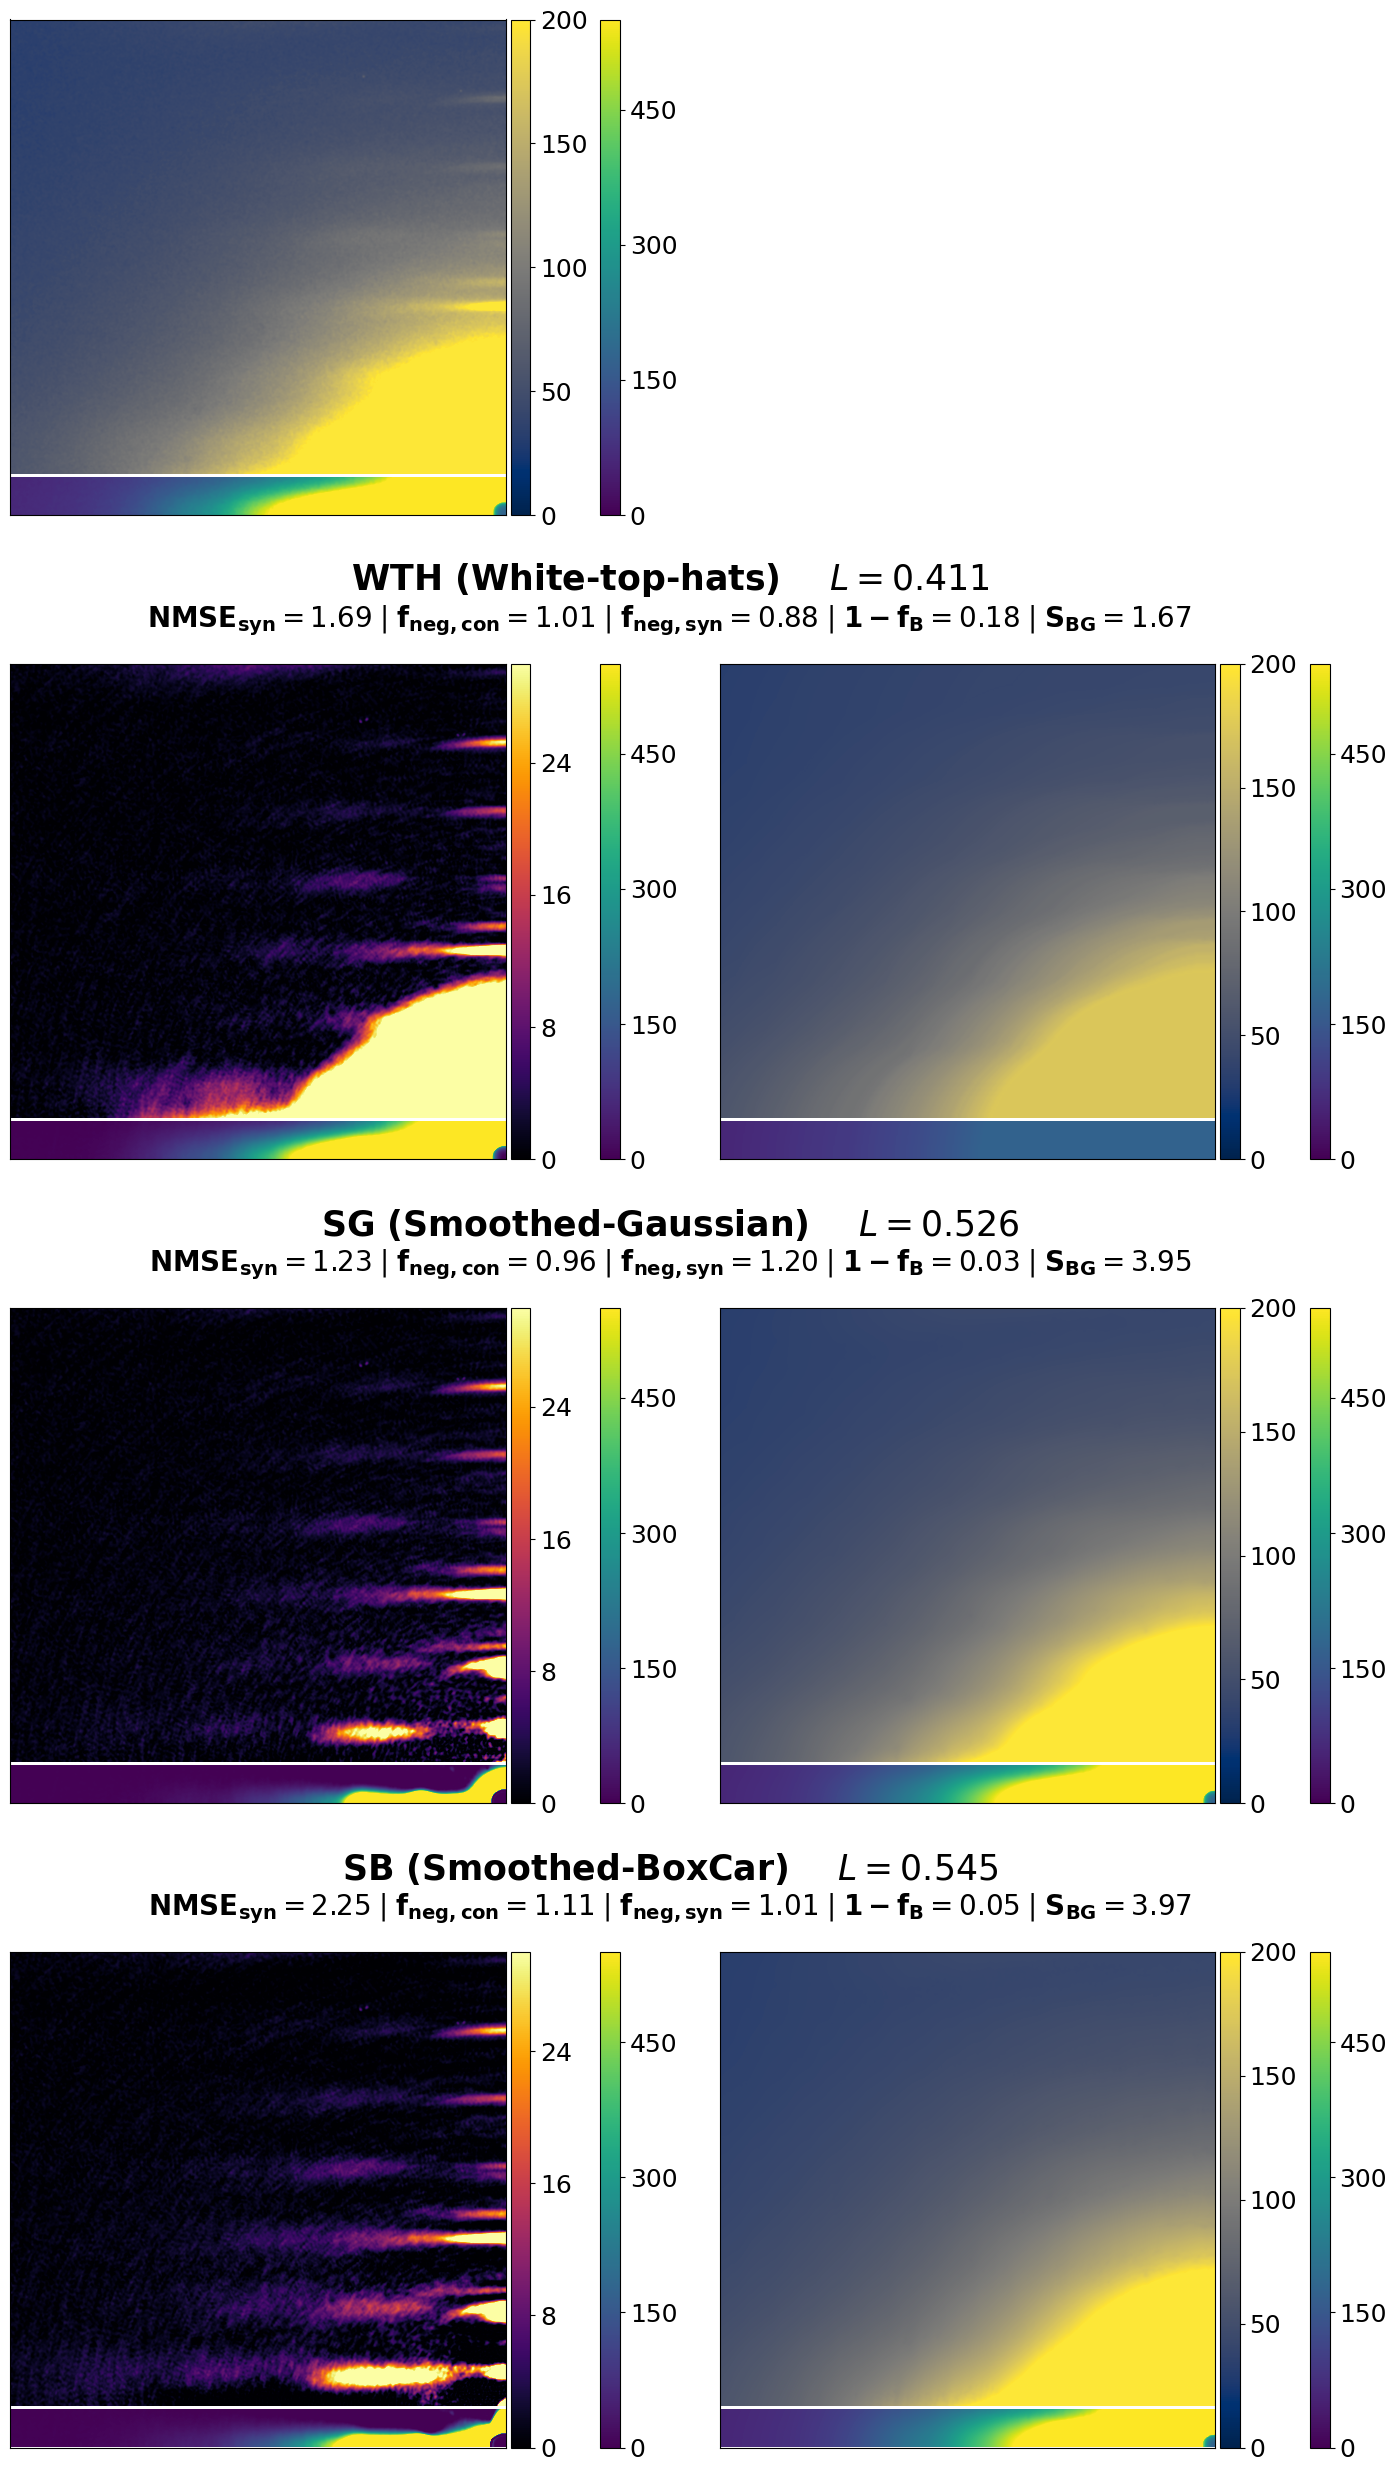
\includegraphics[width=0.88\textwidth]{figs/1_image_Jani_0_left.png}
\end{minipage}\hfill
\begin{minipage}{0.48\textwidth}
    \raggedright
    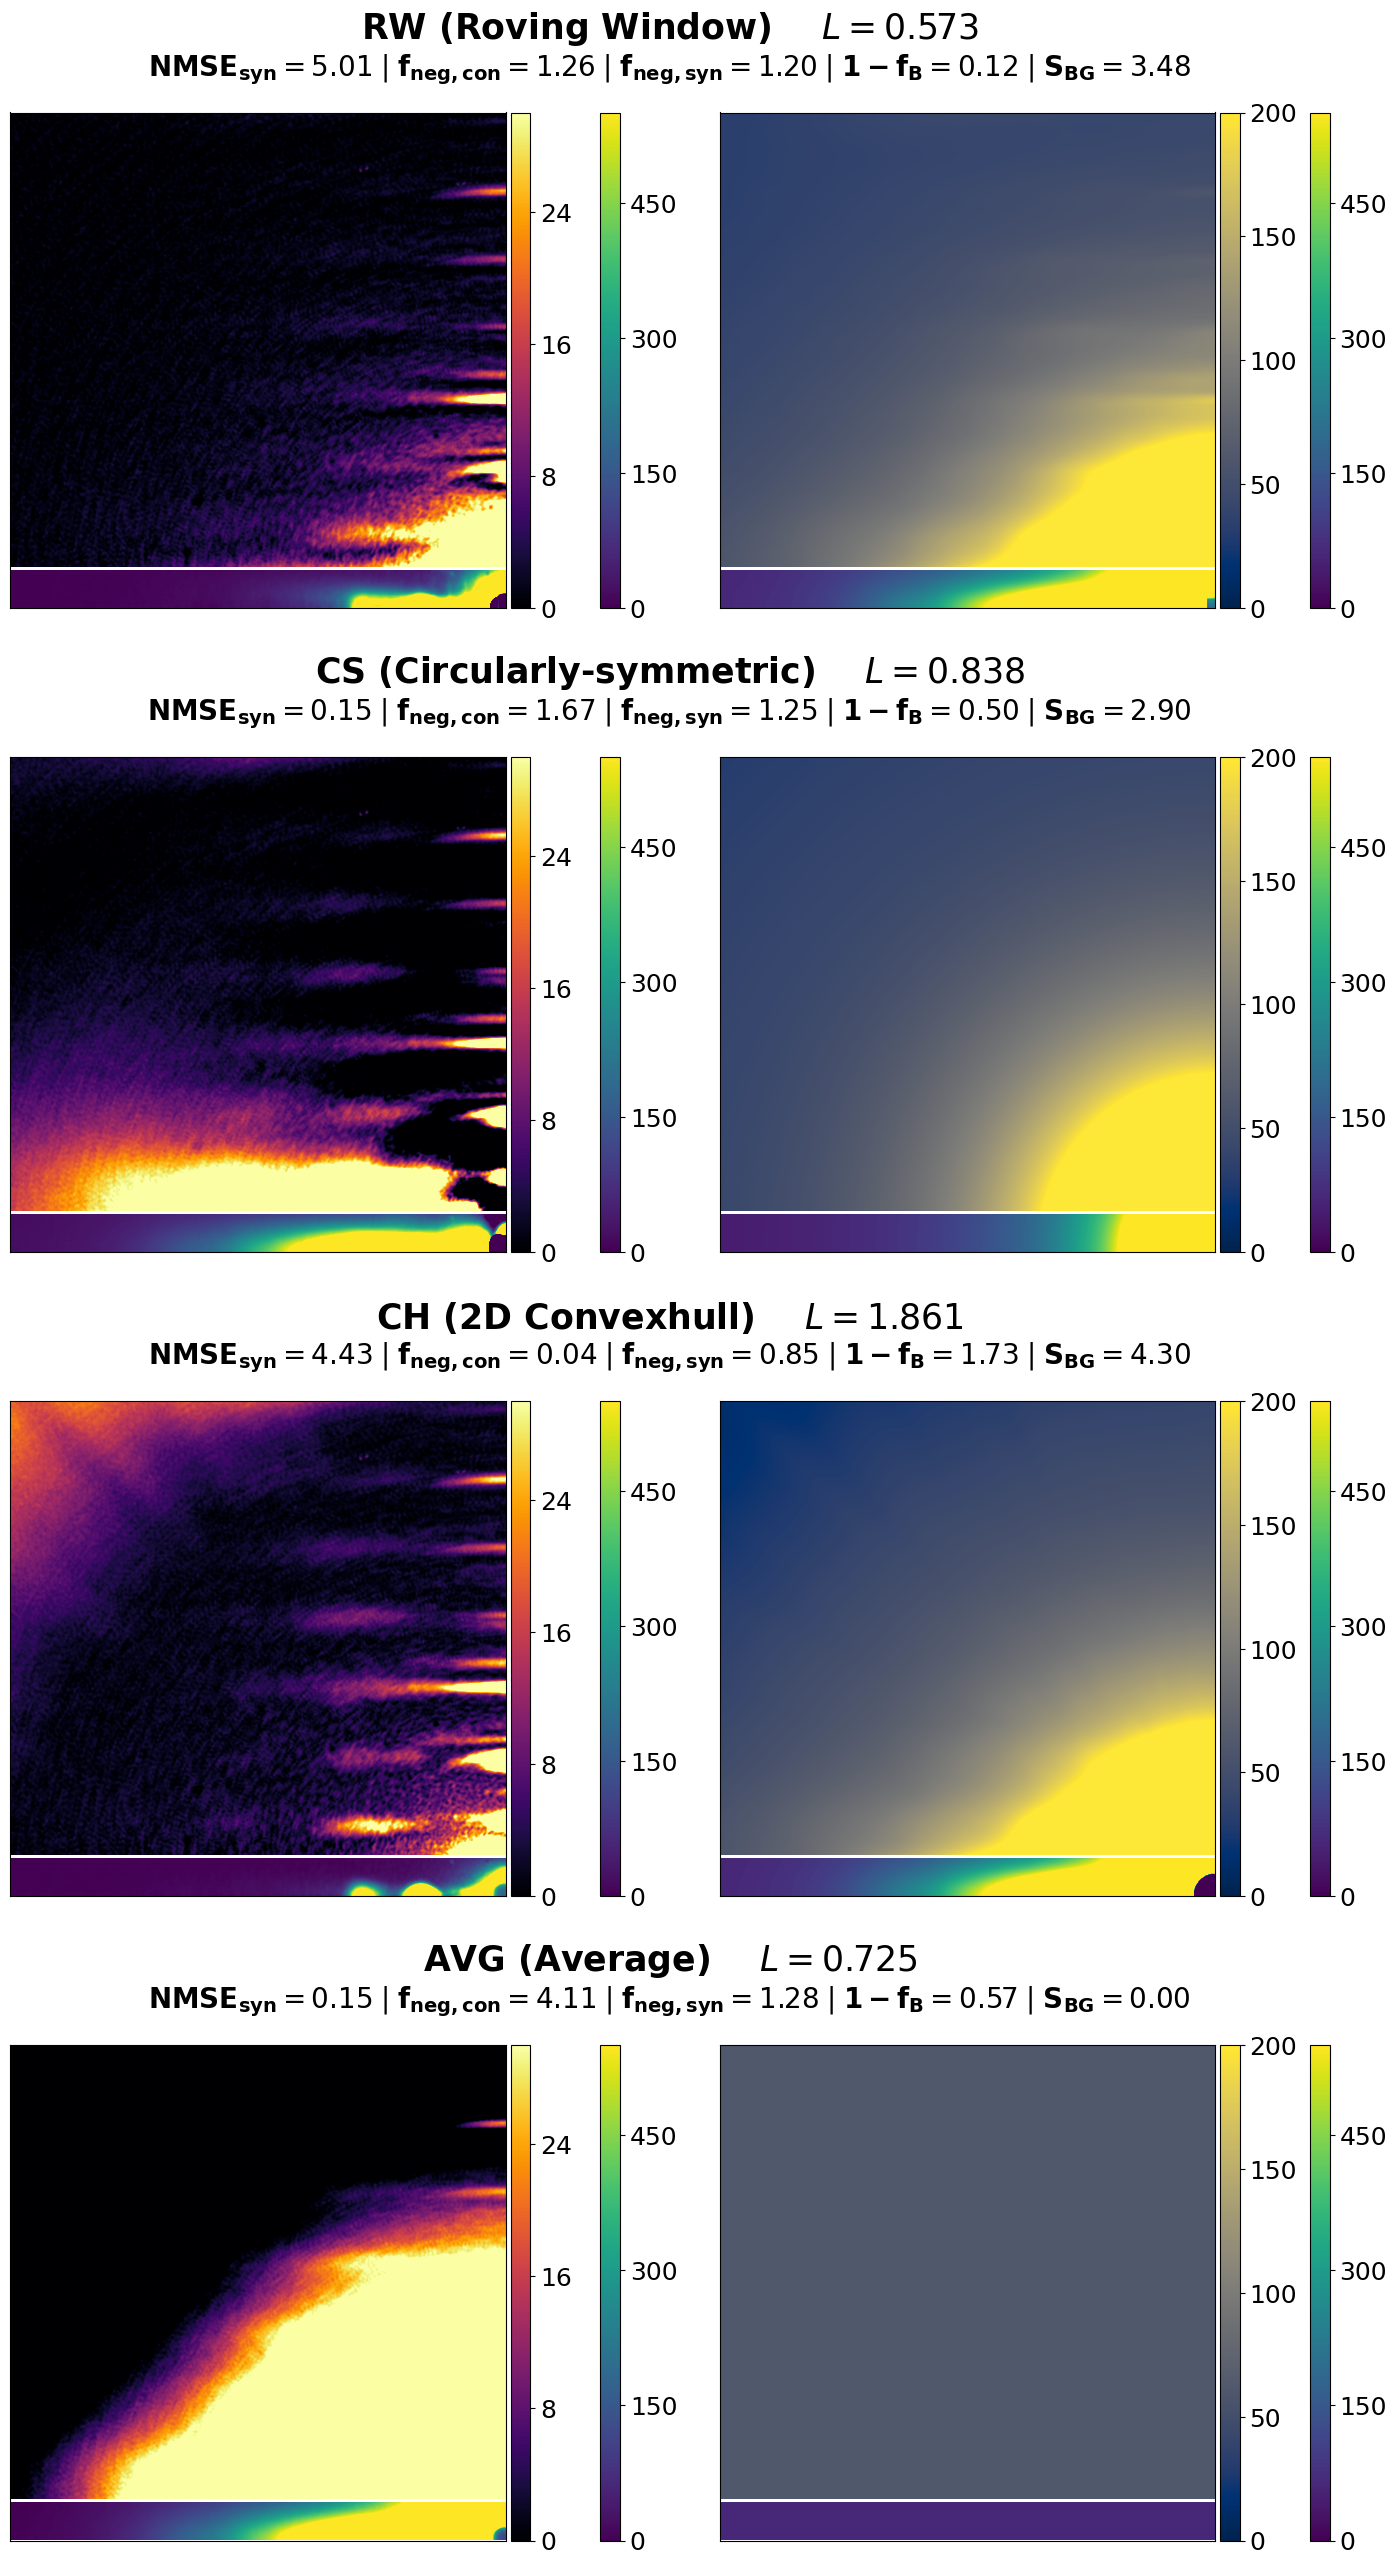
\includegraphics[width=0.88\textwidth]{figs/1_image_Jani_0_right.png}
\end{minipage}
\caption{\footnotesize Visual comparison of background subtraction outcomes for image from dataset 2025\_0402. Top left: original image. Rest: background-sutracted pattern (left), background (right). Two scales are used
for visualization due to high intensity differences between the background, the equatorial streak and the rest of the pattern.}
\label{fig:example_1img_all_bg}
\end{figure}


%%%%%%%%%%%%%%%%%%%%%%%%%%%%%%%%%%%%%%%%%%
%\isPreprints{}{% This command is only used for ``preprints''.
\begin{adjustwidth}{-\extralength}{0cm}
%} % If the paper is ``preprints'', please uncomment this parenthesis.
%\printendnotes[custom] % Un-comment to print a list of endnotes

\reftitle{References}

% References must be numbered in order of appearance in the text (including citations in tables and legends) and listed individually at the end of the manuscript. We recommend preparing the references with a bibliography software package, such as EndNote, ReferenceManager or Zotero, to avoid typing mistakes and duplicated references. Include the digital object identifier (DOI) for all references where available.
% Please provide either the correct journal abbreviation (e.g. according to the “The list of Title Word Abbreviations” https://portal.issn.org/ltwa) or the full name of the journal. 
% Citations and references in the Supplementary Materials are permitted provided that they also appear in the reference list here. 
% In the text, reference numbers should be placed in square brackets [ ] and placed before the punctuation; for example, [1], [1–3] or [1,3]. For embedded citations in the text with pagination, use both parentheses and brackets to indicate the reference number and page numbers; for example, [5] (p. 10), or [6] (pp. 101–105).

%=====================================
% References, variant A: external bibliography
%=====================================
% \bibliography{your_external_BibTeX_file}

%=====================================
% References, variant B: internal bibliography
%=====================================

% ACS format
% \begin{thebibliography}{999}
% % Reference 1
% \bibitem{ref-journal}
% Author~1, T. The title of the cited article. {\em Journal Abbreviation} {\bf 2008}, {\em 10}, 142--149.
% % Reference 2
% \bibitem{ref-book1}
% Author~2, L. The title of the cited contribution. In {\em The Book Title}; Editor 1, F., Editor 2, A., Eds.; Publishing House: City, Country, 2007; pp. 32--58.
% % Reference 3
% \bibitem{ref-book2}
% Author 1, A.; Author 2, B. \textit{Book Title}, 3rd ed.; Publisher: Publisher Location, Country, 2008; pp. 154--196.
% % Reference 4
% \bibitem{ref-unpublish}
% Author 1, A.B.; Author 2, C. Title of Unpublished Work. \textit{Abbreviated Journal Name} year, \textit{phrase indicating stage of publication (submitted; accepted; in press)}.
% % Reference 5
% \bibitem{ref-url}
% Title of Site. Available online: URL (accessed on Day Month Year).
% % Reference 6
% \bibitem{ref-proceeding}
% Author 1, A.B.; Author 2, C.D.; Author 3, E.F. Title of presentation. In Proceedings of the Name of the Conference, Location of Conference, Country, Date of Conference (Day Month Year); Abstract Number (optional), Pagination (optional).
% % Reference 7
% \bibitem{ref-thesis}
% Author 1, A.B. Title of Thesis. Level of Thesis, Degree-Granting University, Location of University, Date of Completion.
% \end{thebibliography}

% ACS format
\begin{thebibliography}{999}
% Reference 1
\bibitem{MaIrving2022}
Ma, W.; Irving, T.C. Small Angle X-ray Diffraction as a Tool for Structural Characterization of Muscle Disease. {\em Int. J. Mol. Sci.} {\bf 2022}, {\em 23}, 3052.
% Reference 2
\bibitem{squire2003ccp13_software}
Squire, J.; Al-Khayat, H.; Arnott, S.; Crawshaw, J.; Denny, R.; Diakun, G.; Dover, D.; Forsyth, T.; He, A.; Knupp, C.; Mant, G.; Rajkumar, G.; Rodman, M.; Shotton, M.; Windle, A. New CCP13 Software and the Strategy Behind Further Developments: Stripping and Modelling of Fibre Diffraction Data. {\em Fibre Diffr. Rev.} {\bf 2003}, {\em 11}, 7--19.
% Reference 3
\bibitem{He2018}
He, B.B. \textit{Two-Dimensional X-ray Diffraction}, 2nd ed.; Wiley: Hoboken, NJ, USA, 2018.
% Reference 4
\bibitem{jarvis1973convex_hull}
Jarvis, R.A. On the Identification of the Convex Hull of a Finite Set of Points in the Plane. {\em Inf. Process. Lett.} {\bf 1973}, {\em 2}, 18--21.
% Reference 5
\bibitem{lee2019musclex}
Lee, X.; Jiratrakanvong, J.; Nikseresht, G.; Irving, T.; Agam, G. MuscleX, Version 1.14.12, 2019. Available online: https://doi.org/10.5281/zenodo.3360909 (accessed on 3 July 2026).
% Reference 6
\bibitem{rajkumar2007fibrefix}
Rajkumar, G.; Al-Khayat, H.A.; Eakins, F.; Knupp, C.; Squire, J.M. The CCP13 FibreFix Program Suite: Semi-Automated Analysis of Diffraction Patterns from Non-Crystalline Materials. {\em J. Appl. Cryst.} {\bf 2007}, {\em 40}, 178--184.

% Reference 7
\bibitem{IvanovaMakowski1998}
Ivanova, M.I.; Makowski, L. Iterative Low-Pass Filtering for Estimation of the Background in Fiber Diffraction Patterns. {\em Acta Crystallogr. A} {\bf 1998}, {\em 54}, 626--631.
% Reference 8
\bibitem{GonzalezWoodsDIP4e}
Gonzalez, R.C.; Woods, R.E. \textit{Digital Image Processing}, 4th ed.; Pearson: New York, NY, USA, 2018.
% Reference 9
\bibitem{PolarBackground2024}
Guo, P.; Zheng, X.; Jiang, J.; Yin, S.; Zhang, C.; Yang, B.; Cui, Y.; Yang, T.; Gu, Y.; Li, X.; Zhang, X. Polar Coordinate-Based Background Removal Algorithm for 2D X-ray Scattering Data. {\em Rev. Sci. Instrum.} {\bf 2024}, {\em 95}, 125109.
% Reference 10
\bibitem{WaveletBiomedOptExpress2021}
H\"upfel, M.; Kobitski, A.Y.; Zhang, W.; Nienhaus, G.U. Wavelet-Based Background and Noise Subtraction for Fluorescence Microscopy Images. {\em Biomed. Opt. Express} {\bf 2021}, {\em 12}, 969--980.
% Reference 11
\bibitem{renedecotret2017baseline}
Ren\'e de Cotret, L.P.; Siwick, B.J. A General Method for Baseline-Removal in Ultrafast Electron Powder Diffraction Data Using the Dual-Tree Complex Wavelet Transform. {\em Struct. Dyn.} {\bf 2017}, {\em 4}, 044004.
% Reference 12
\bibitem{Sternberg1983}
Sternberg, S.R. Biomedical Image Processing. {\em Computer} {\bf 1983}, {\em 16}, 22--34.
% Reference 13
\bibitem{ArangurenCarmona2020}
Aranguren Carmona, R.; Agam, G.; Irving, T. Background Subtraction in Diffraction X-ray Images Using Deep CNN. {\em Electron. Imaging} {\bf 2020}, {\em 32}, 344-1--344-6.
% Reference 14
\bibitem{Buerger1940}
Buerger, M.J. The Correction of X-ray Diffraction Intensities for Lorentz and Polarization Factors. {\em Proc. Natl. Acad. Sci. USA} {\bf 1940}, {\em 26}, 637--642.
% Reference 15
\bibitem{Denny1995}
Denny, R. Fibre Diffraction Spot Profiles and the Lorentz Correction. {\em Fibre Diffr. Rev.} {\bf 1995}, {\em 5}, 23--25.
% Reference 16
\bibitem{JiratrakanvongEtAl2024}
Jiratrakanvong, J.; Shao, J.; Li, J.; Menendez Alvarez, M.; Li, X.; Das, P.; Nikseresht, G.; Miskin, N.; Huo, R.; Nabon, J.; Leduc, T.; Zhang, E.; Ma, W.; Agam, G.; Irving, T.C. MuscleX: Data Analysis Software for Fiber Diffraction Patterns from Muscle. {\em J. Synchrotron Radiat.} {\bf 2024}, {\em 31}, 1401--1408.
% Reference 17
\bibitem{MurthyZeroGrubb1997}
Murthy, N.S.; Zero, K.; Grubb, D.T. Full-Pattern Analysis of Two-Dimensional Small-Angle Scattering Data from Oriented Polymers Using Elliptical Coordinates. {\em Polymer} {\bf 1997}, {\em 38}, 1021--1028.
\end{thebibliography}




% If authors have biography, please use the format below
%\section*{Short Biography of Authors}
%\bio
%{\raisebox{-0.35cm}{\includegraphics[width=3.5cm,height=5.3cm,clip,keepaspectratio]{Definitions/author1.pdf}}}
%{\textbf{Firstname Lastname} Biography of first author}
%
%\bio
%{\raisebox{-0.35cm}{\includegraphics[width=3.5cm,height=5.3cm,clip,keepaspectratio]{Definitions/author2.jpg}}}
%{\textbf{Firstname Lastname} Biography of second author}

% For the MDPI journals use author-date citation, please follow the formatting guidelines on http://www.mdpi.com/authors/references
% To cite two works by the same author: \citeauthor{ref-journal-1a} (\citeyear{ref-journal-1a}, \citeyear{ref-journal-1b}). This produces: Whittaker (1967, 1975)
% To cite two works by the same author with specific pages: \citeauthor{ref-journal-3a} (\citeyear{ref-journal-3a}, p. 328; \citeyear{ref-journal-3b}, p.475). This produces: Wong (1999, p. 328; 2000, p. 475)

%%%%%%%%%%%%%%%%%%%%%%%%%%%%%%%%%%%%%%%%%%
%% for journal Sci
%\reviewreports{\\
%Reviewer 1 comments and authors’ response\\
%Reviewer 2 comments and authors’ response\\
%Reviewer 3 comments and authors’ response
%}
%%%%%%%%%%%%%%%%%%%%%%%%%%%%%%%%%%%%%%%%%%
\PublishersNote{}
%\isPreprints{}{% This command is only used for ``preprints''.
\end{adjustwidth}
%} % If the paper is ``preprints'', please uncomment this parenthesis.
\end{document}

